\chapter{Georeferencing}
\section{Georeferencing with point cloud}

It is possible to set session as ground truth.
Thus, optimization process (Pose GRAPH SLAM) will not change its poses.
Other sessions can be aligned against ground truth session by adding edges.

\begin{figure}[H]
	\centering
	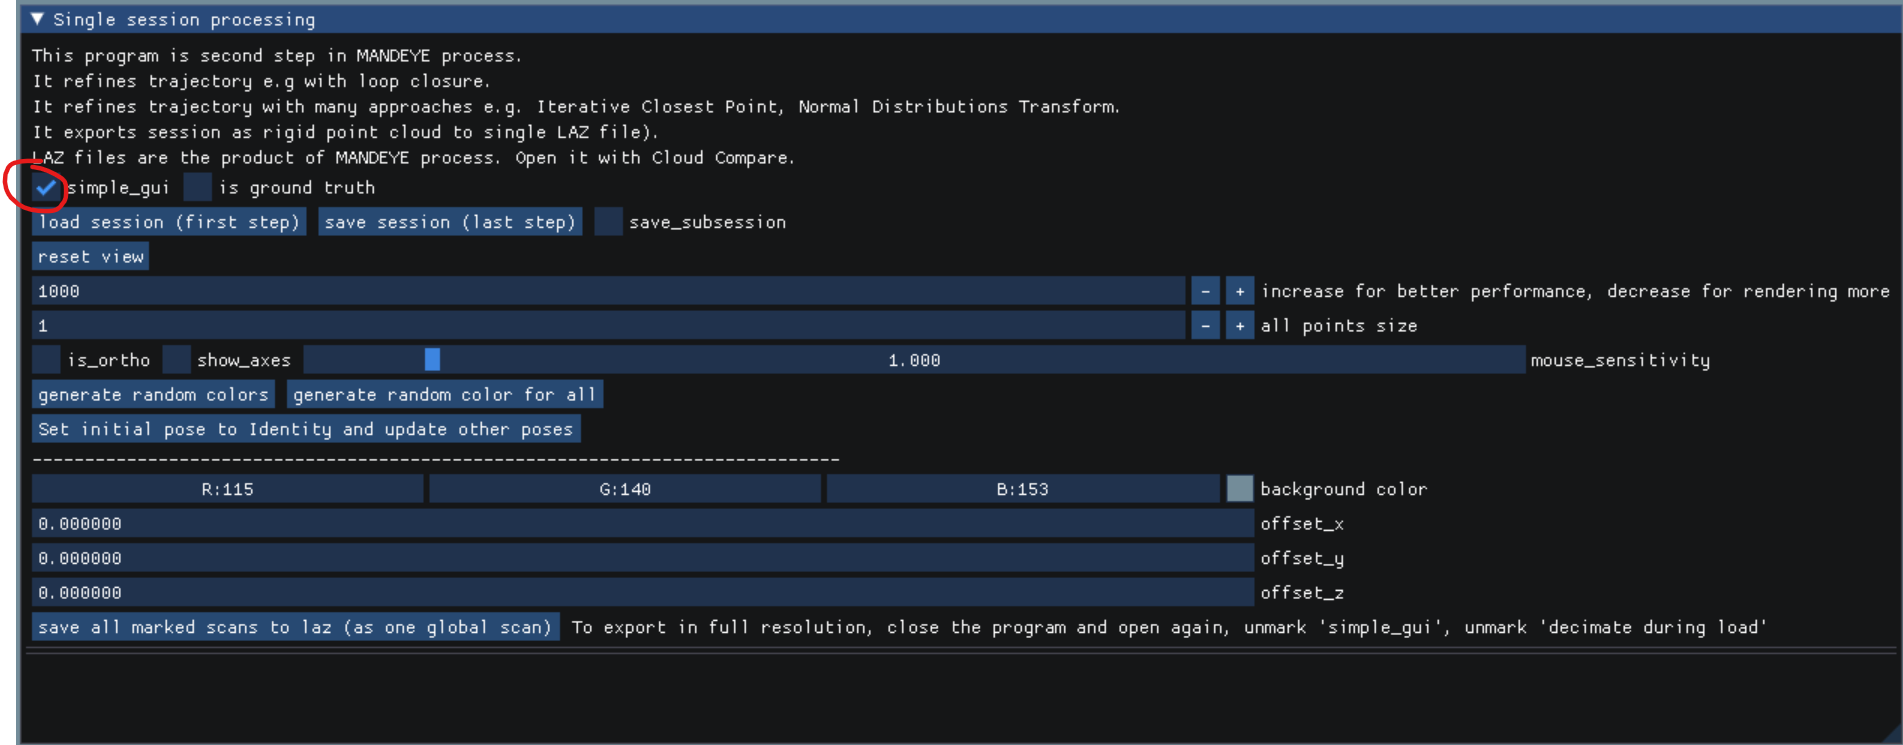
\includegraphics[width=\textwidth]{g1.png}
	\caption{Use multi view tls registration step2 program to open TLS files.}
	\label{fig:g1}
\end{figure}

\begin{figure}[H]
	\centering
	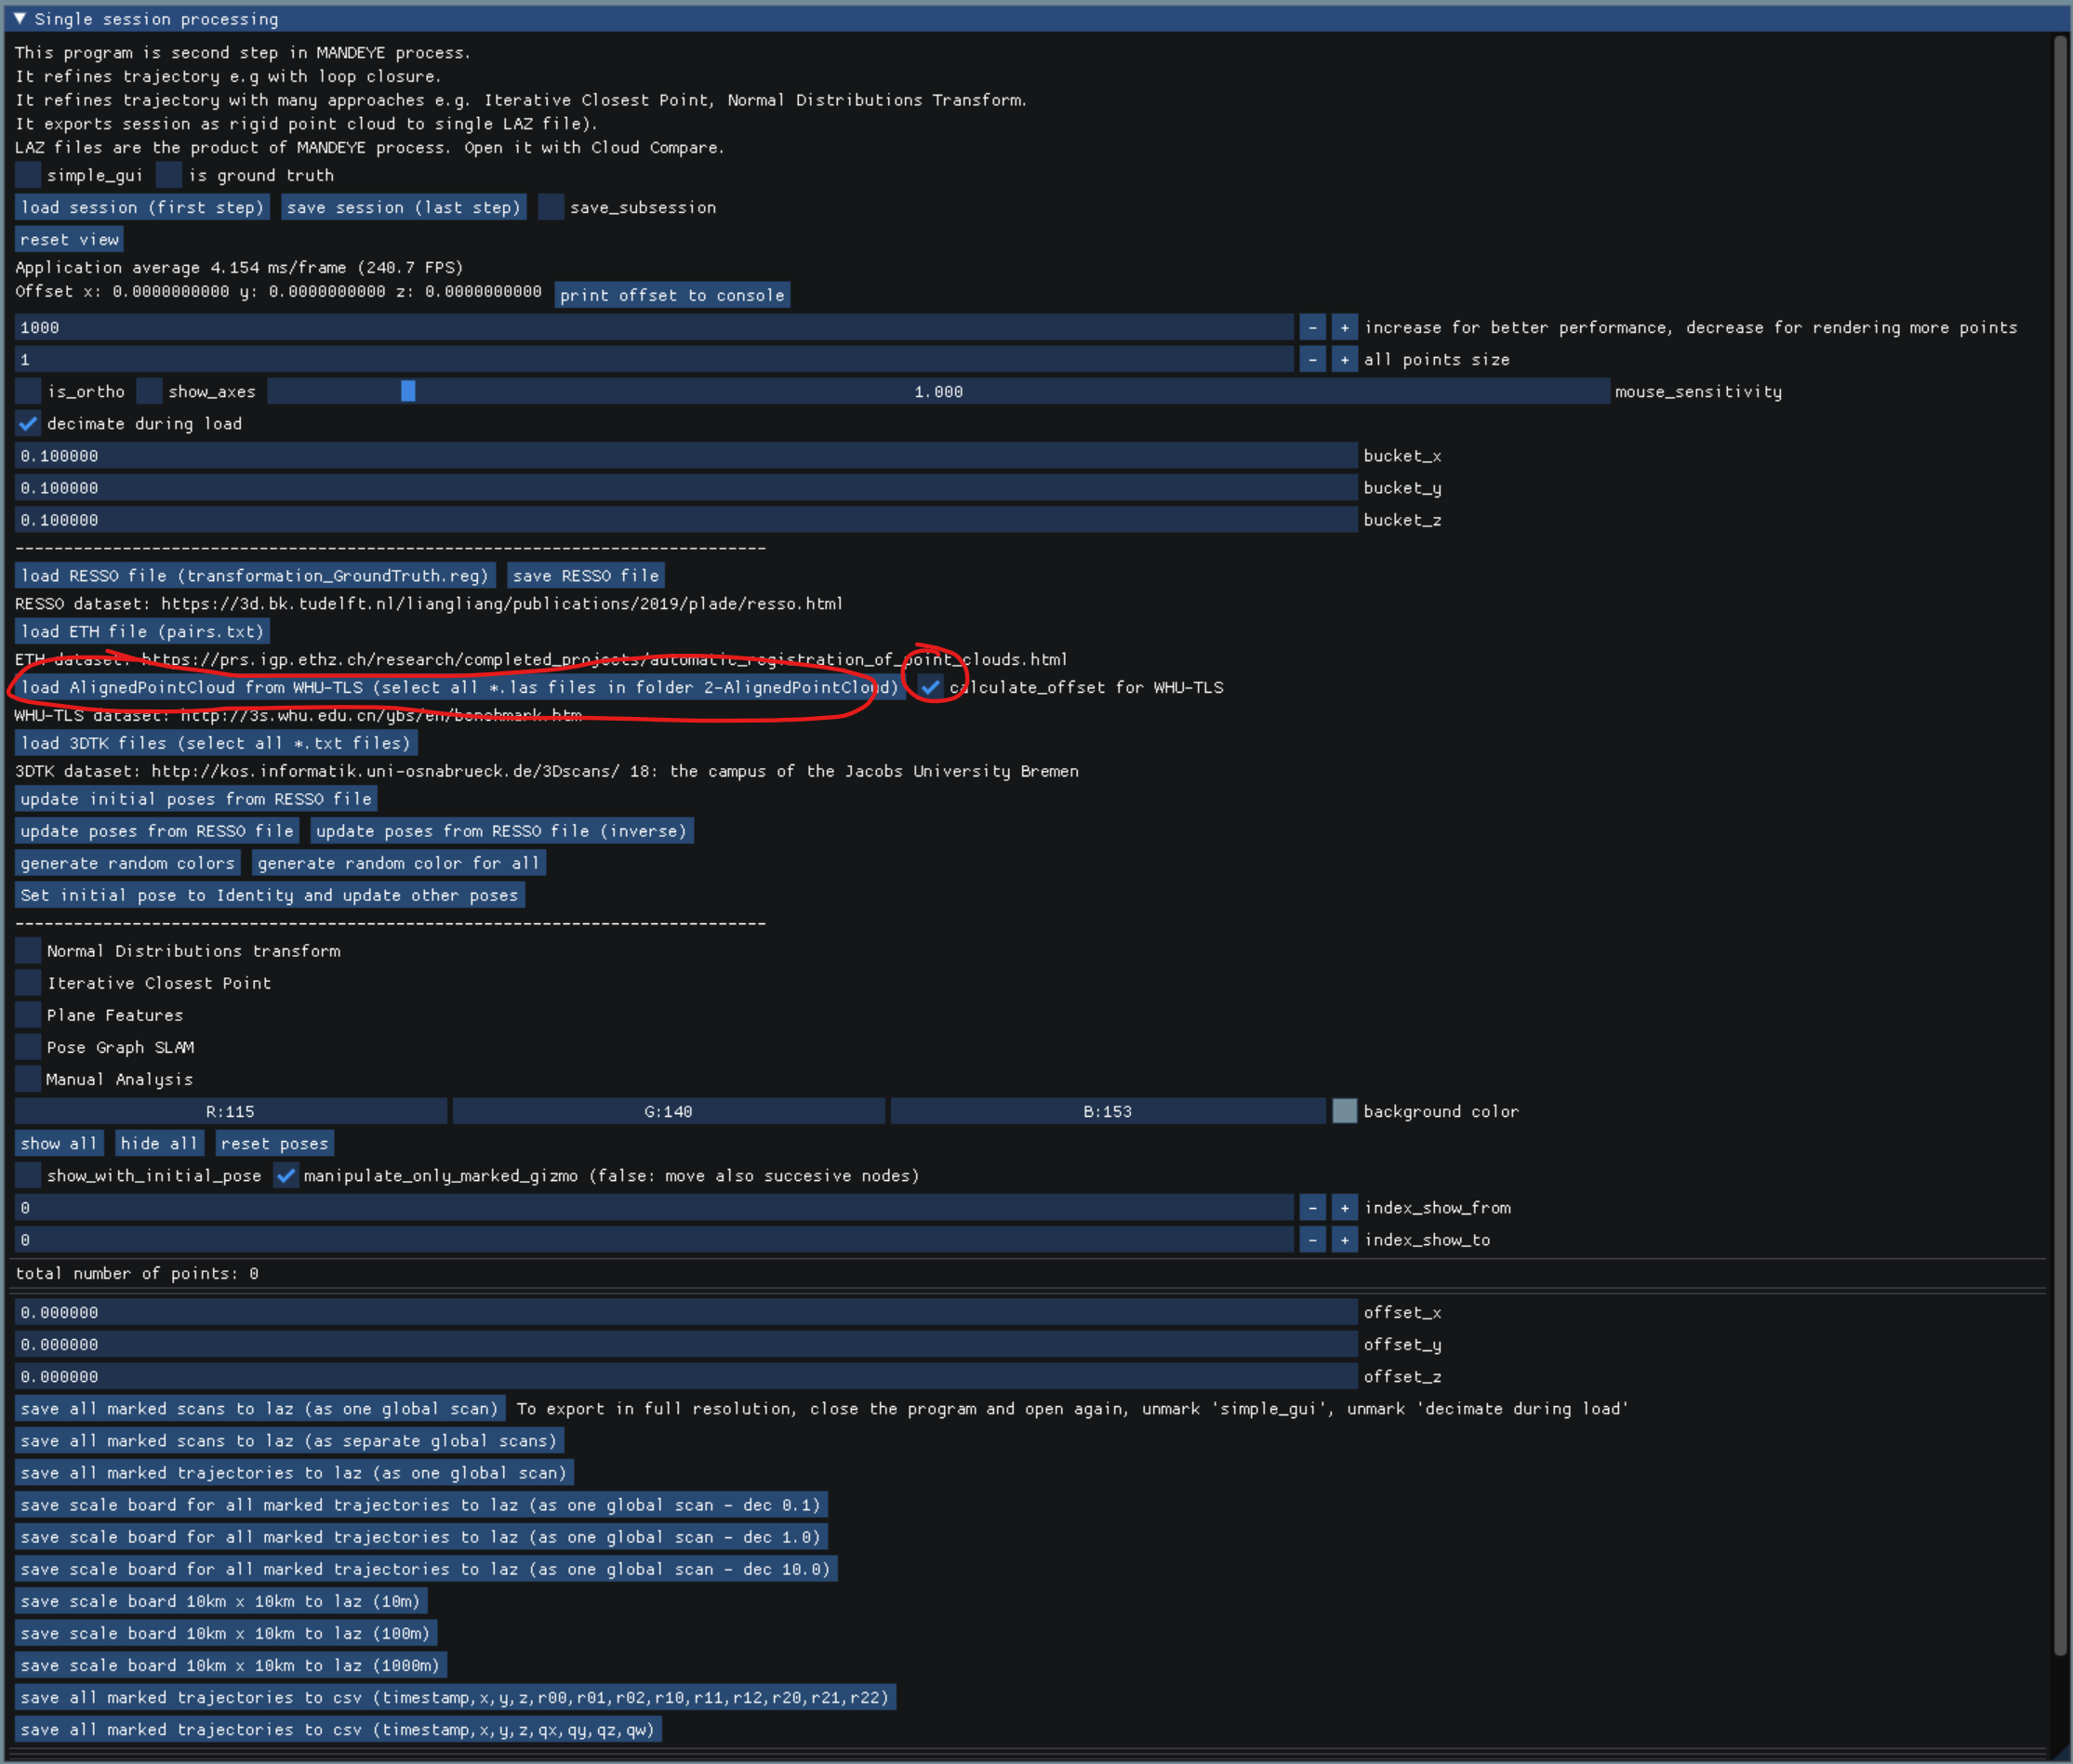
\includegraphics[width=\textwidth]{g2.png}
	\caption{Mark calculate offset for WHU-TLS, load AlignedPointCloud from WHU-TLS (select all *.las/laz files in folder)}
	\label{fig:g2}
\end{figure}

\begin{figure}[H]
	\centering
	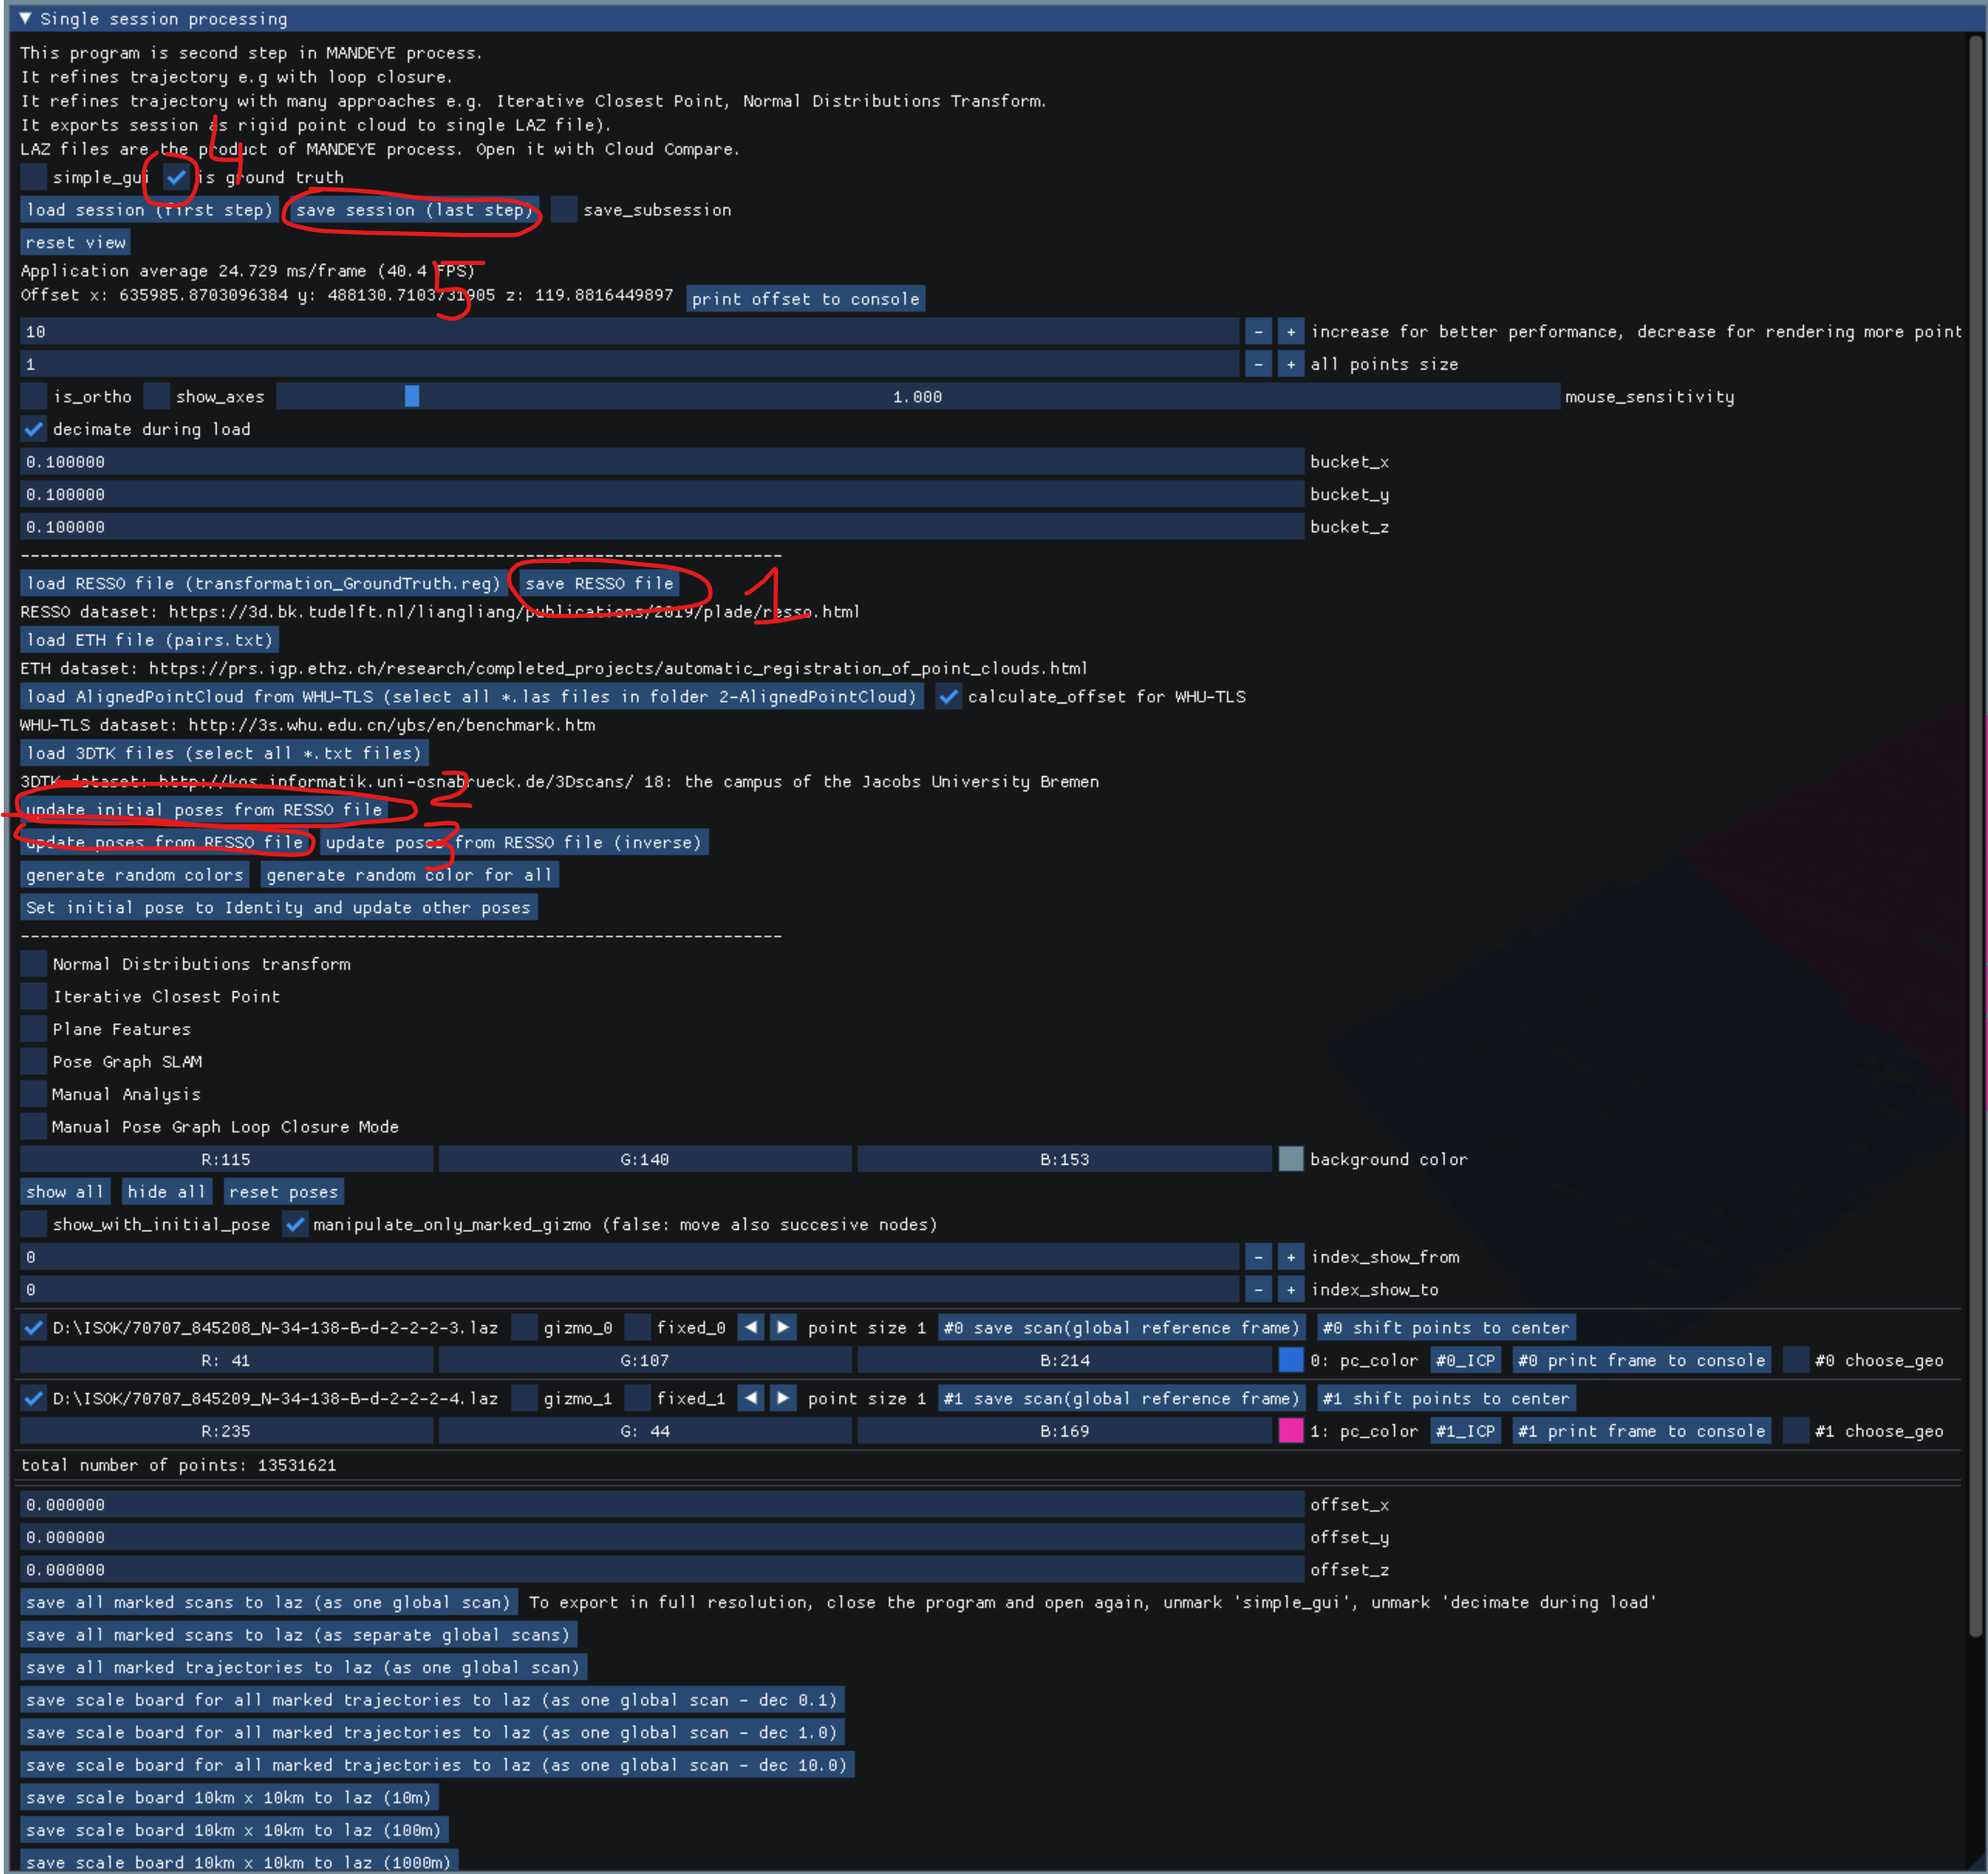
\includegraphics[width=\textwidth]{g3.png}
	\caption{1: save RESSO file, 2: update initial poses from RESSO file (select file from 1), 3: update poses from RESSO file (select file from 1), 4: set checkbox is ground truth, 5: save session.}
	\label{fig:g3}
\end{figure}

\section{Georeferencing with WGS84toCartesian}
\label{Georeferencing_with_WGS84toCartesian}
It uses \url{https://github.com/chrberger/WGS84toCartesian/tree/master} WGS84toCartesian.
It is a small and efficient library written in modern C++ library to convert WGS84 latitude/longitude positions to/from Cartesian positions using Mercator projection.
If You have MANDEYE with GNSS receiver, then it saves data in gnssXXXX.gnss files.
This is ASCII file with\\
---\\
timestamp lat lon alt hdop satelites-tracked height age time fix-quality\\
---\
\begin{figure}[H]
	\centering
	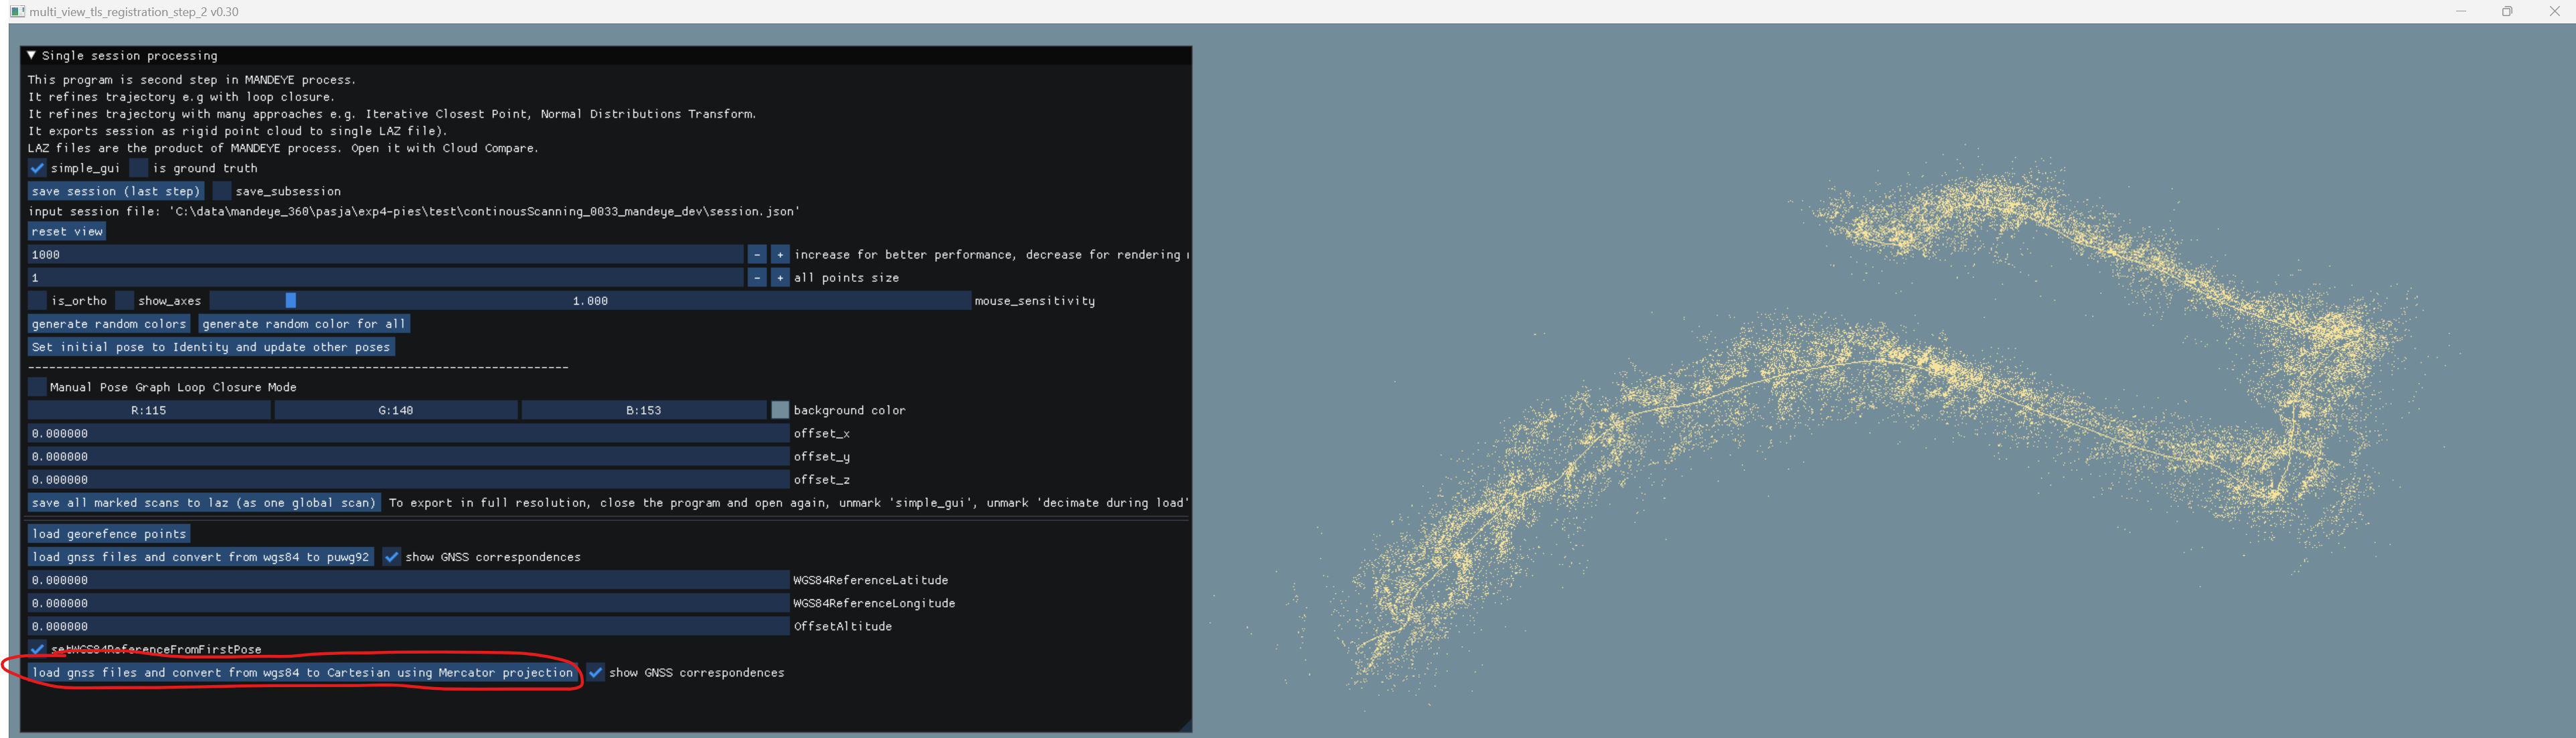
\includegraphics[width=\textwidth]{geo0.png}
	\caption{Georeferencing step 1: load gnss files and convert from wgs84 to Cartesian using Mercator projection.}
	\label{fig:geo0}
\end{figure}

\begin{figure}[H]
	\centering
	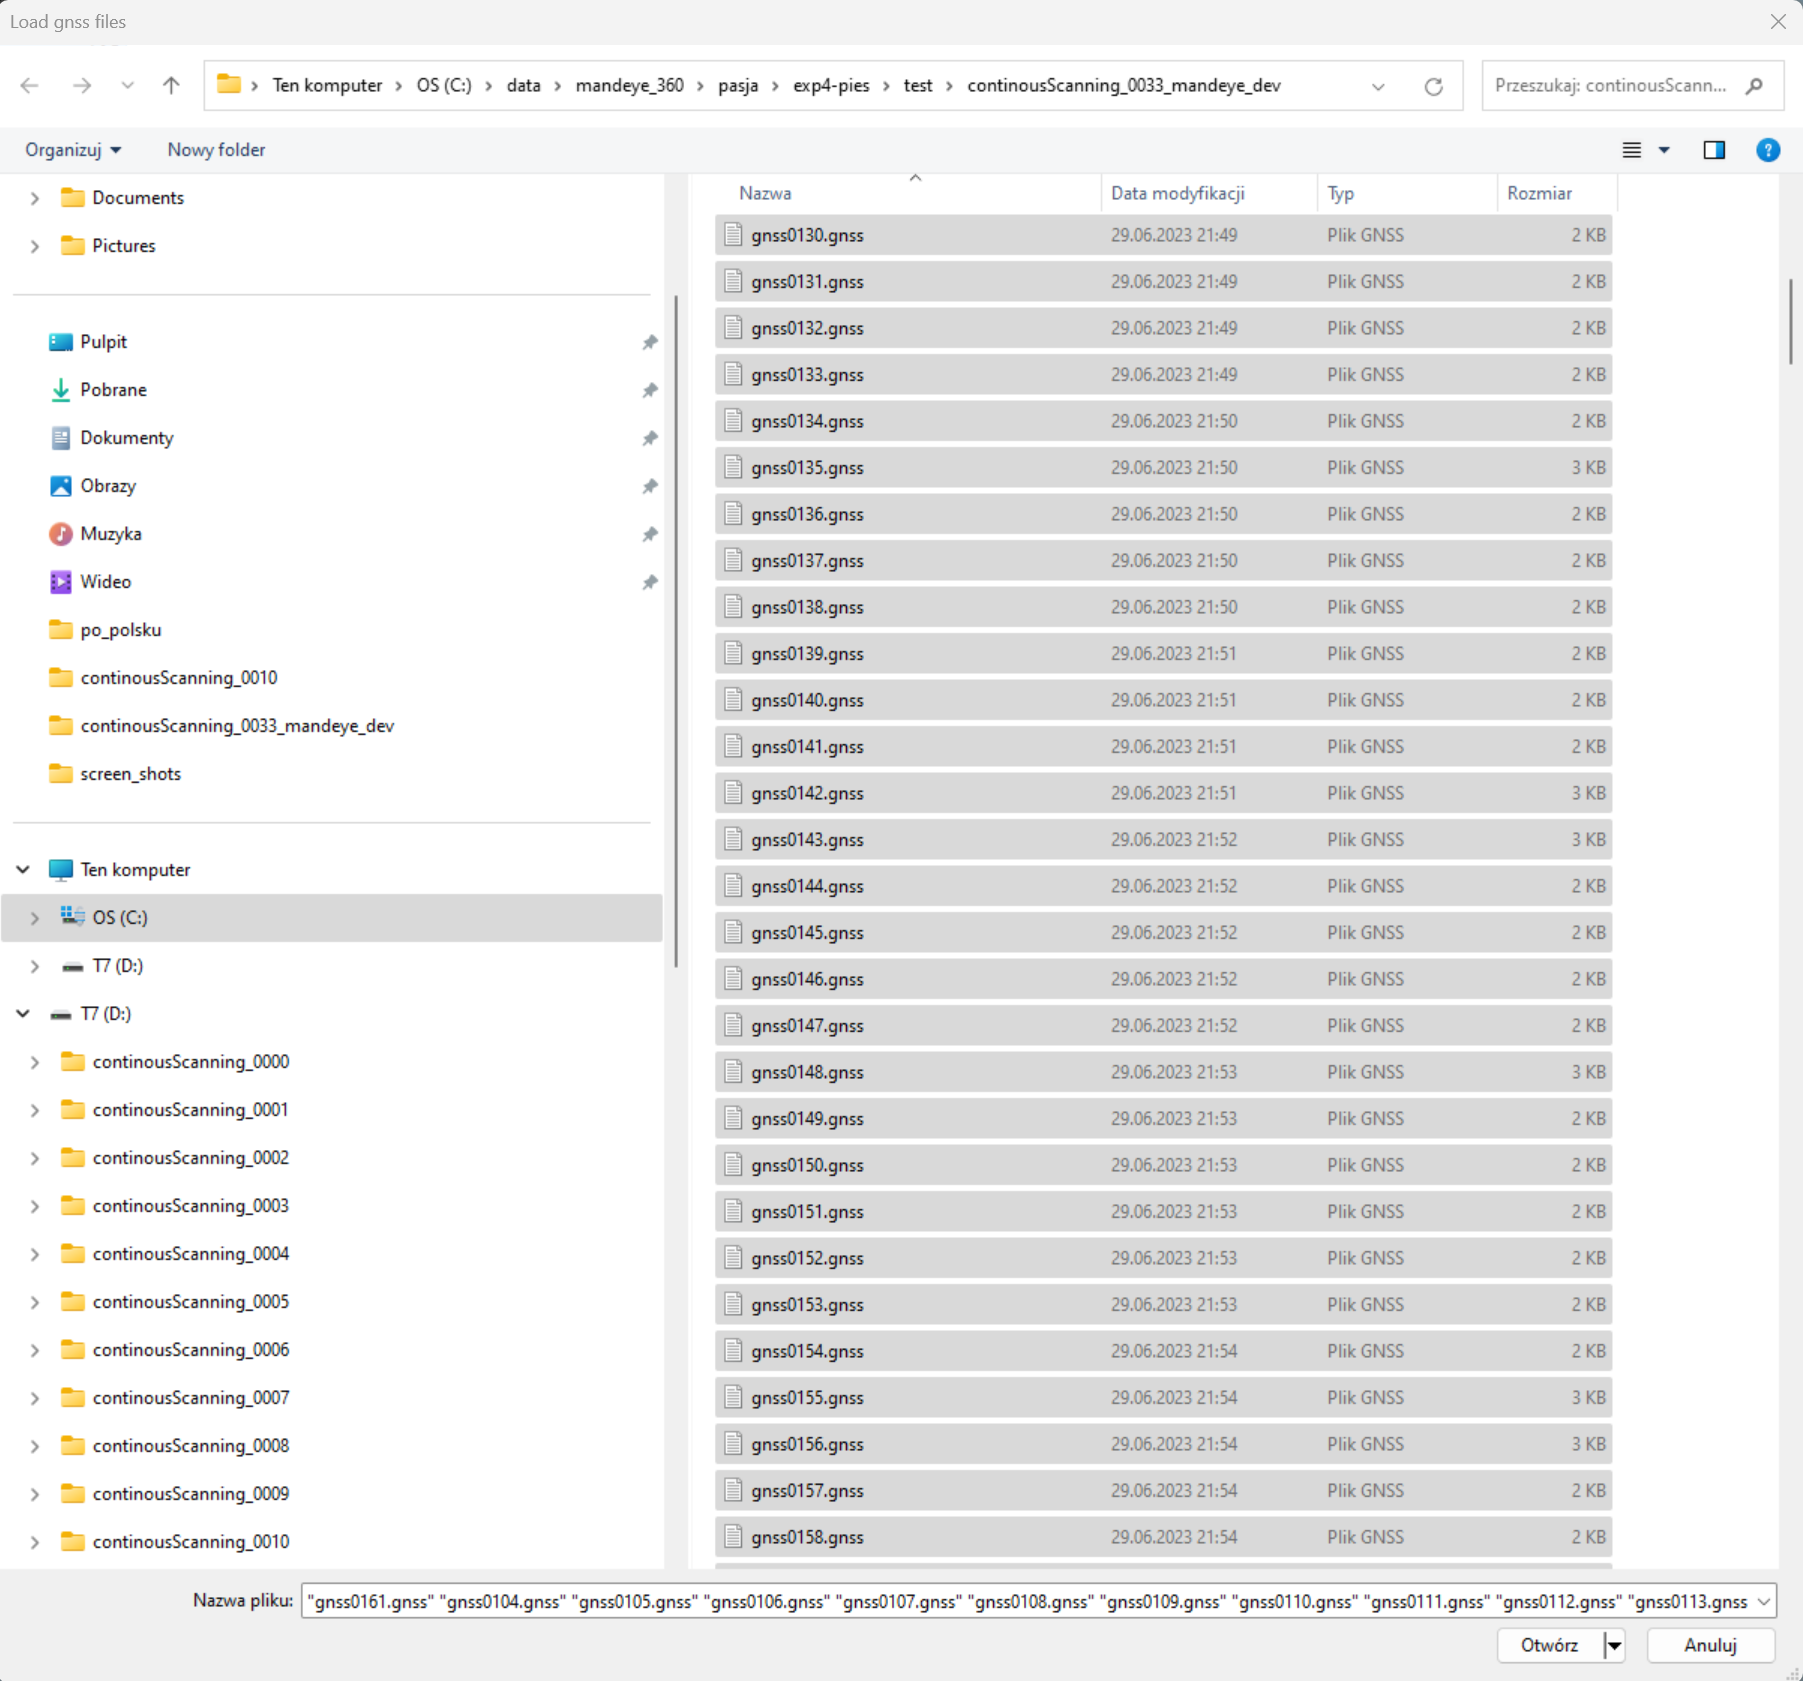
\includegraphics[width=\textwidth]{geo1.png}
	\caption{Georeferencing step 2: mark all gnss files and load.}
	\label{fig:geo1}
\end{figure}

\begin{figure}[H]
	\centering
	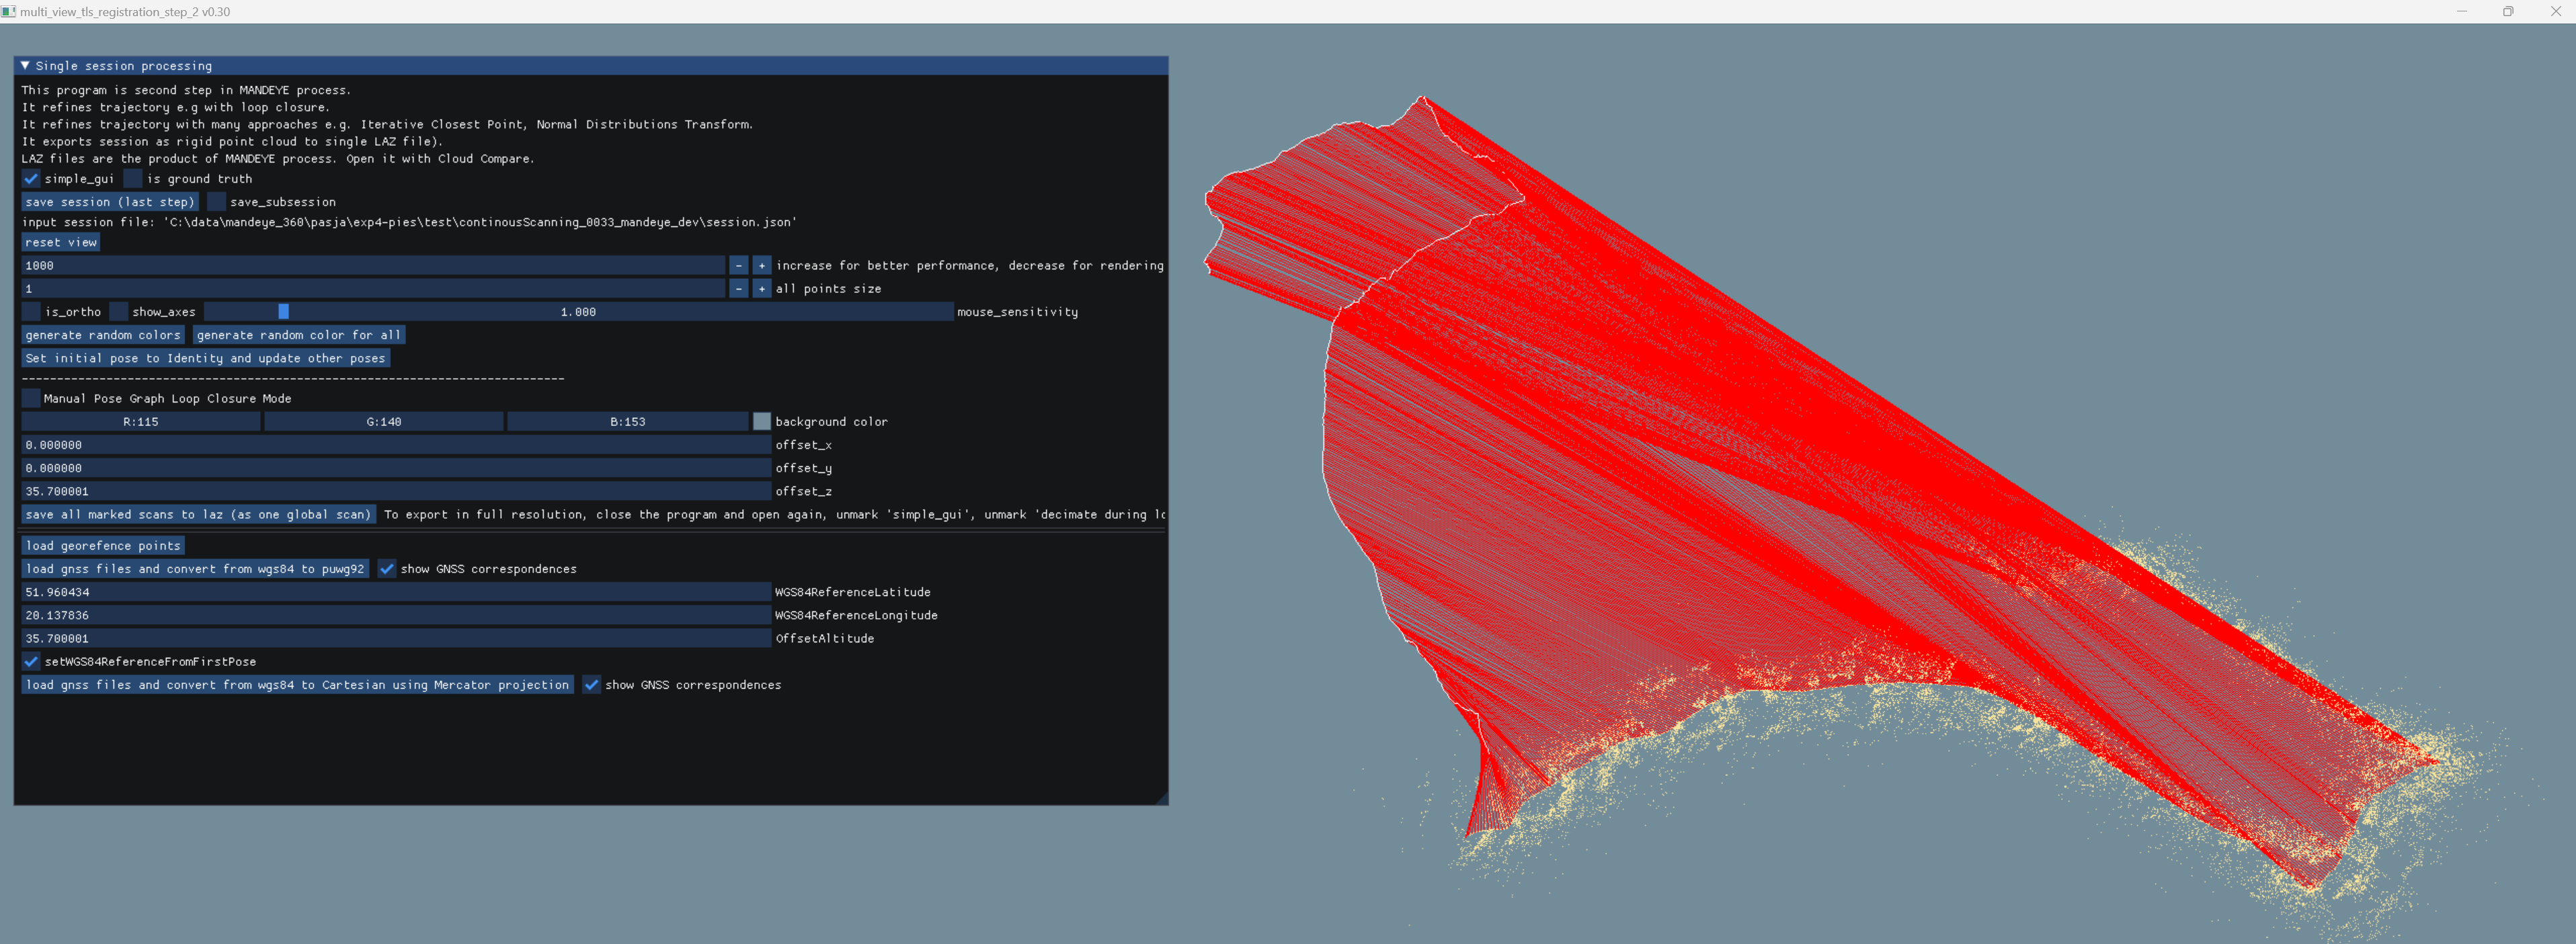
\includegraphics[width=\textwidth]{geo2.png}
	\caption{Georeferencing step 3: check/uncheck 'show GNSS correspondences' to see gnss-poses correspondences. Remark: You can use gizmo for manual initial trajectory to GNSS alignment.}
	\label{fig:geo2}
\end{figure}

\begin{figure}[H]
	\centering
	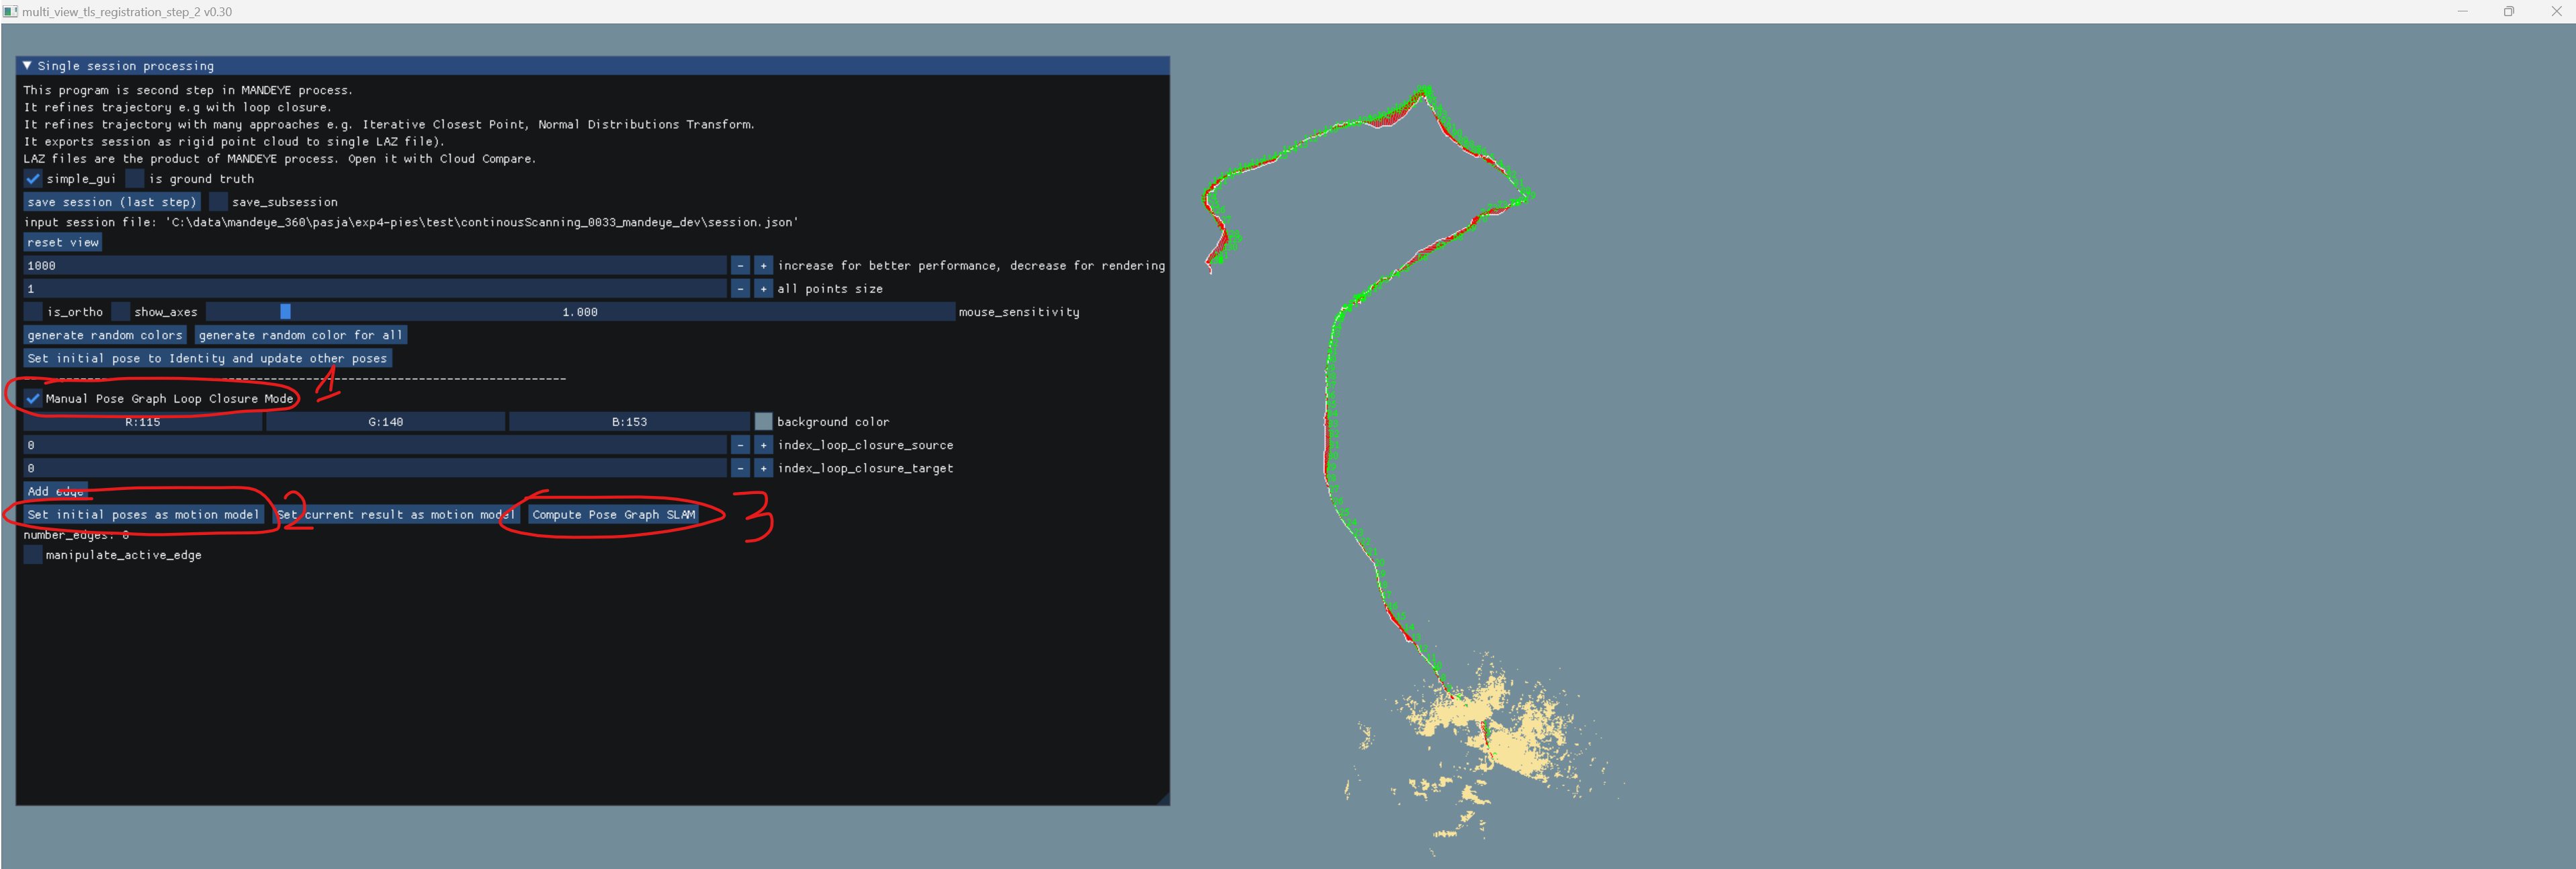
\includegraphics[width=\textwidth]{geo3.png}
	\caption{Georeferencing step 4: Check Manual Pose Graph Loop Closure Mode, then set initial poses as motion model, then Compute Pose Graph SLAM.}
	\label{fig:geo3}
\end{figure}
\pagebreak

\textbf{Below is an example of how to download and create ground truth data from exemplary ALS data (free polish ALS data available as part of ISOK: \url{http://www.gugik.gov.pl/projekty/isok/produkty}) with scans prepared through HDMapping software.}
Figures from \ref{fig:34} to \ref{fig:38} serve only as an example of how the process of gathering and preparing ALS data may look like.

To download ALS data Geoportal site will be used - \url{https://www.geoportal.gov.pl}.

\begin{figure}[H]
	\centering
	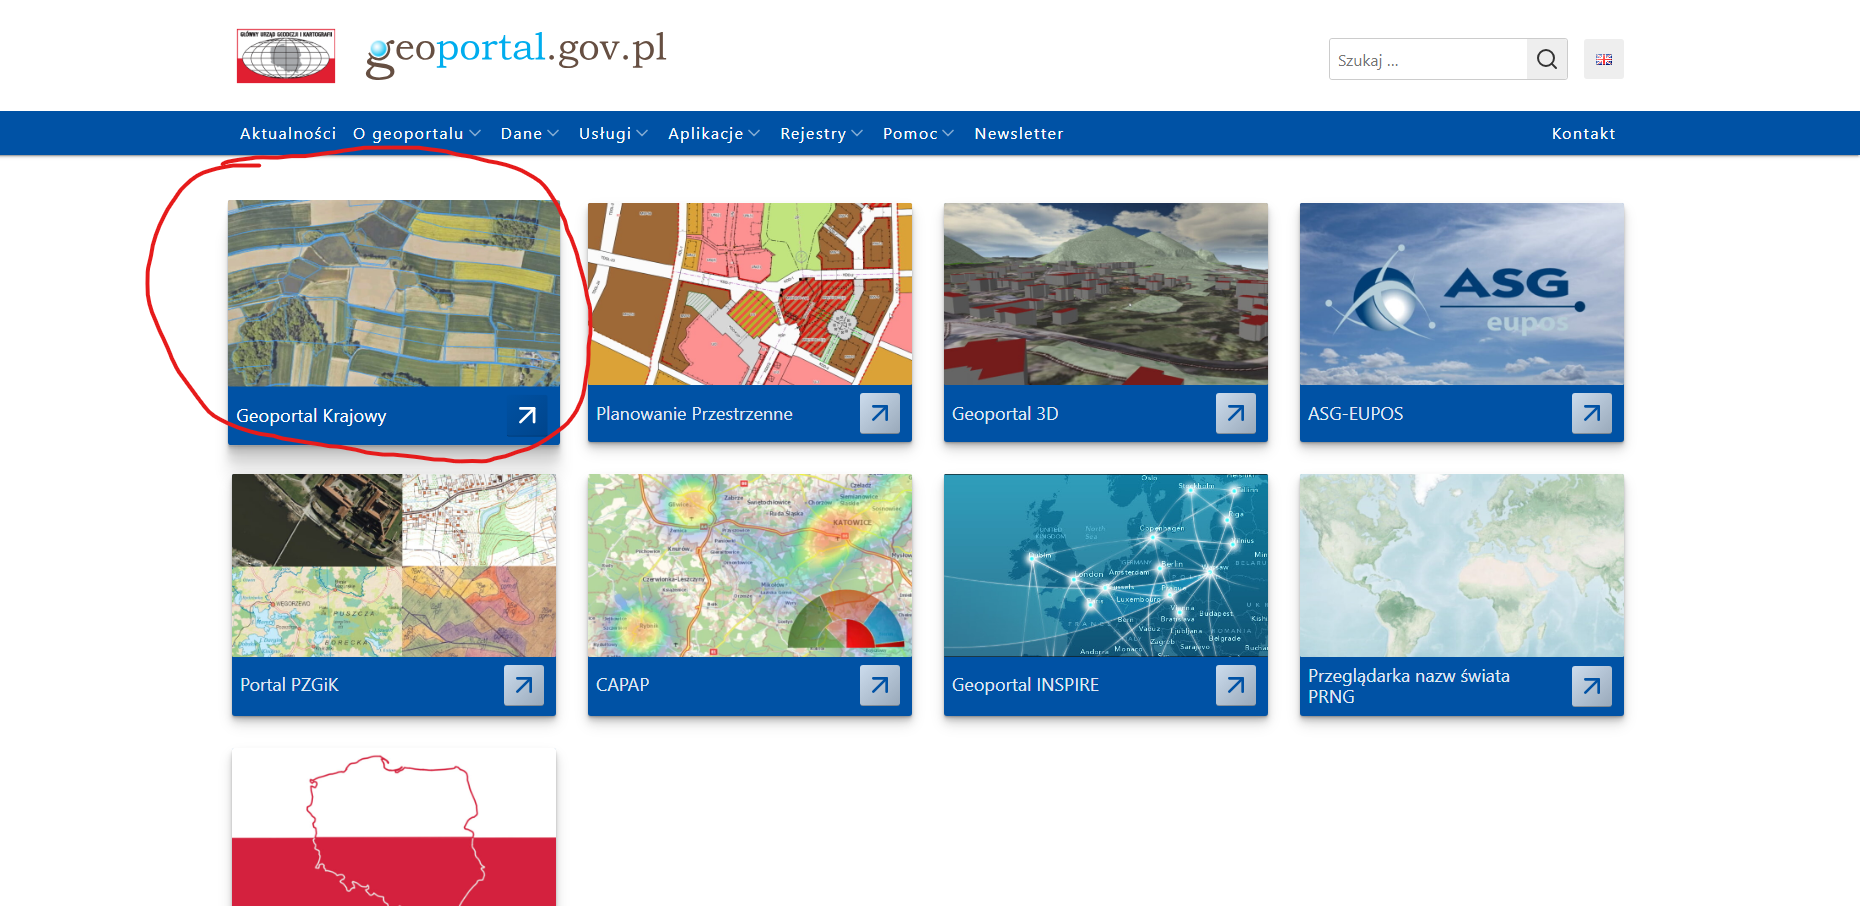
\includegraphics[width=\textwidth]{ISOK1.png}
	\caption{After \url{https://www.geoportal.gov.pl} site is loaded choose Geoportal krajowy tab.}
	\label{fig:34}
\end{figure}

\begin{figure}[H]
	\centering
	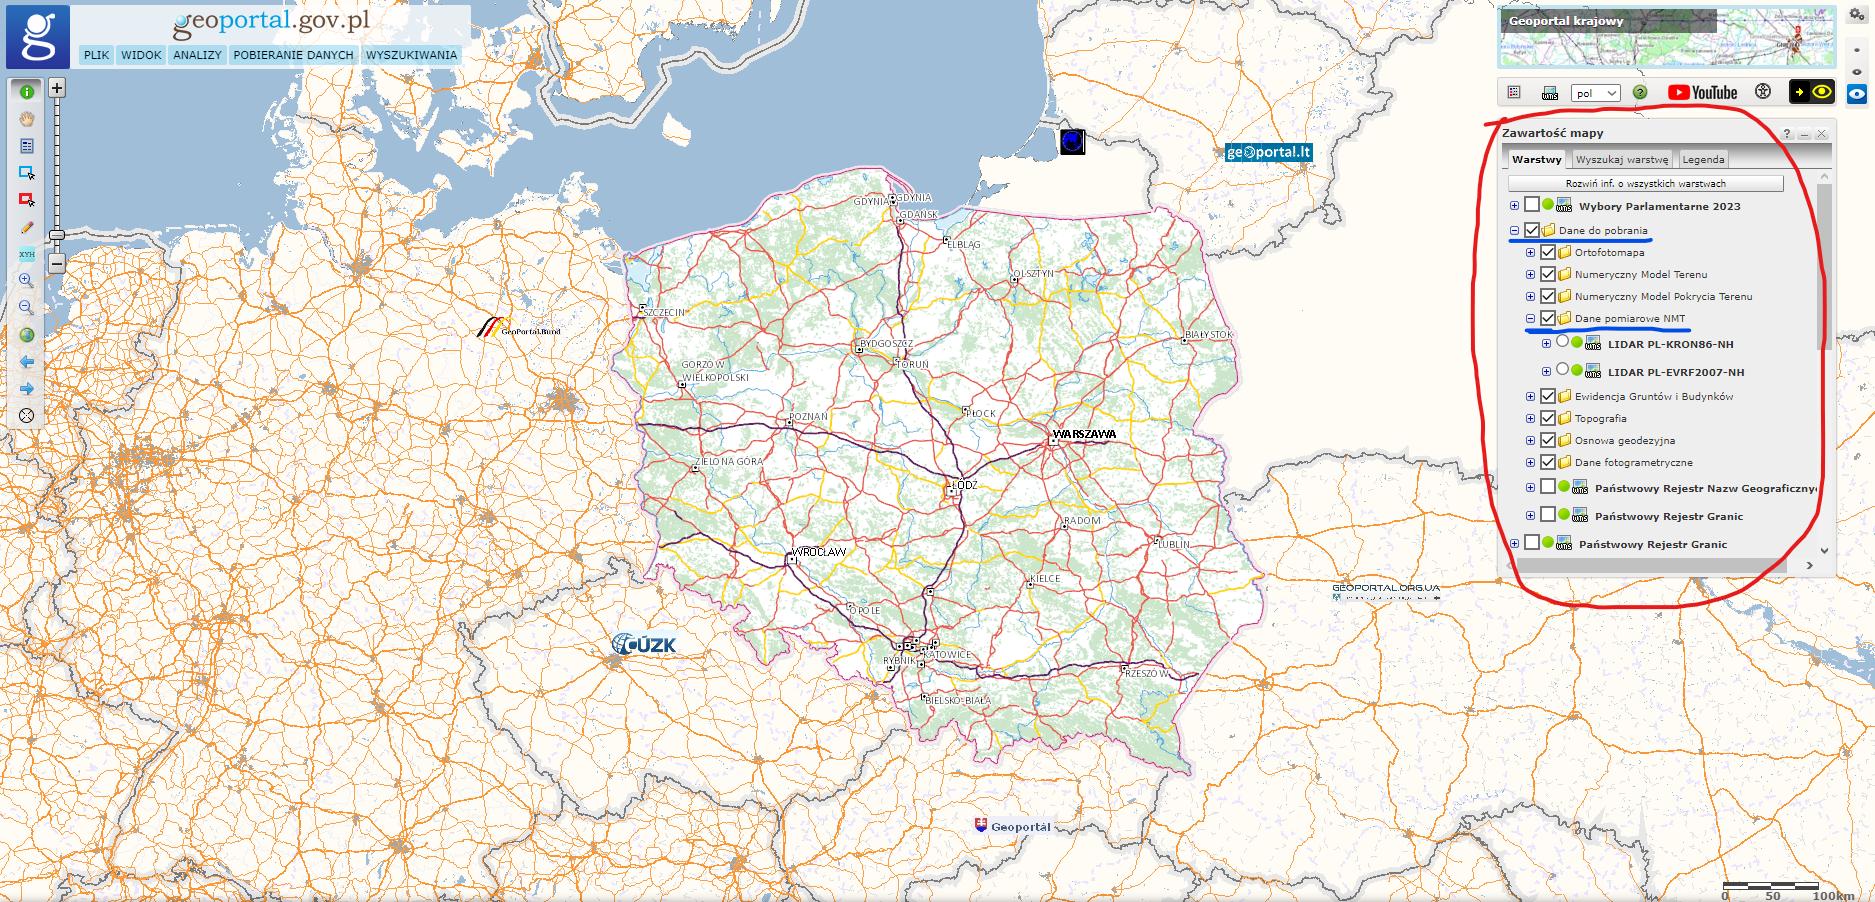
\includegraphics[width=\textwidth]{ISOK2.png}
	\caption{After Geoportal has loaded, on the right side of the screen select Dane do pobrania, then Dane pomiarowe NMT, where 2 options are possible.}
	\label{fig:35}
\end{figure}

\begin{figure}[H]
	\centering
	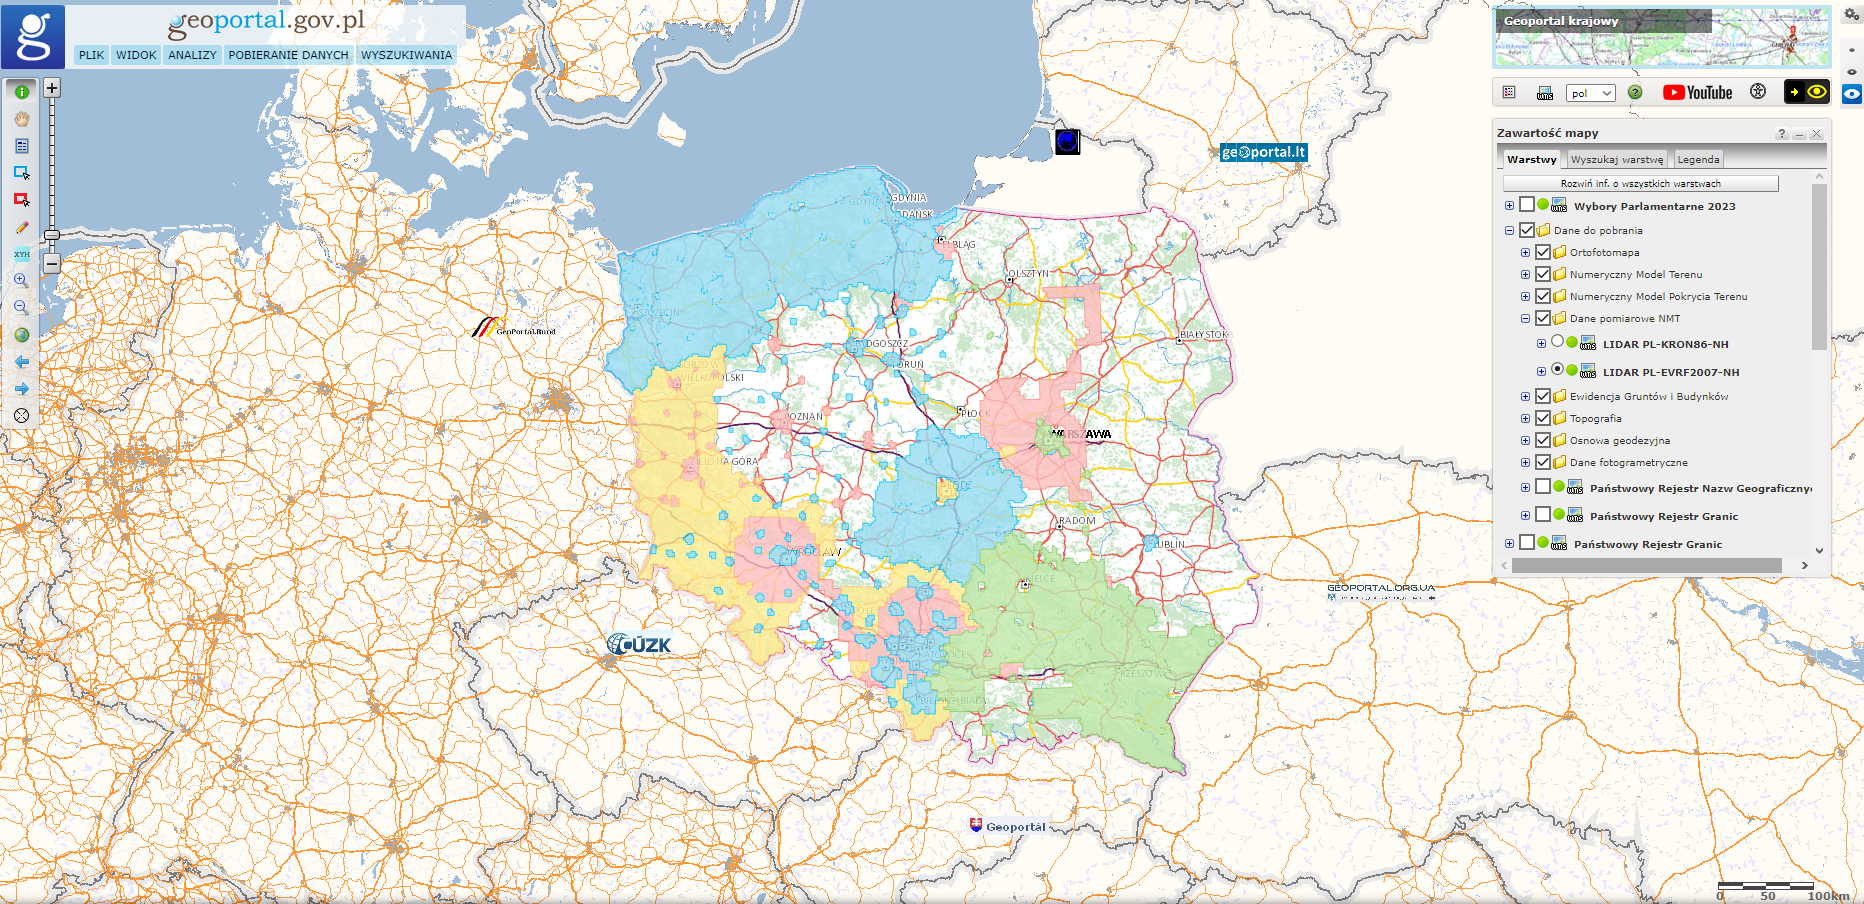
\includegraphics[width=\textwidth]{ISOK3.png}
	\caption{Whenever it is possible EVRF LIDAR version should be chosen over KRON36 version, as the former is more current than the latter. As can be seen on the screen there are parts without EVRF version and in such cases KRON86 is the only option.}
	\label{fig:36}
\end{figure}

\begin{figure}[H]
	\centering
	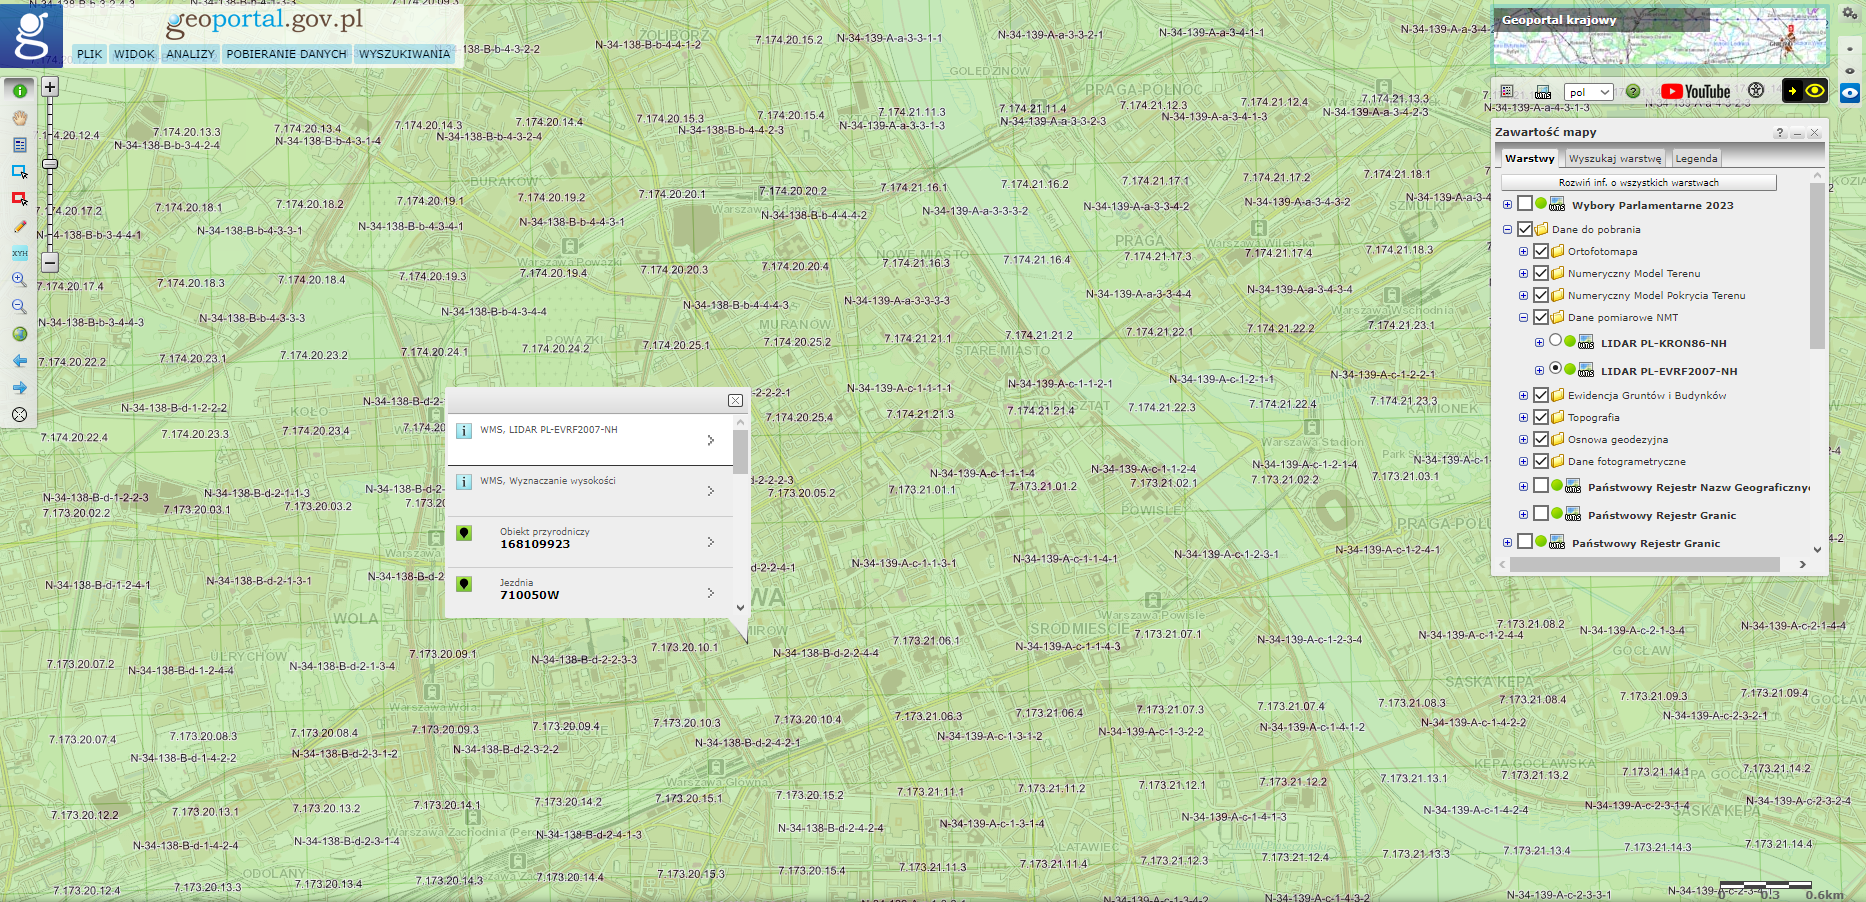
\includegraphics[width=\textwidth]{ISOK4.png}
	\caption{When LIDAR has been chosen zoom in to the map until tiles are seen. To download simply click on the tile with left mouse button and choose WMS, LIDAR.}
	\label{fig:37}
\end{figure}

\begin{figure}[H]
	\centering
	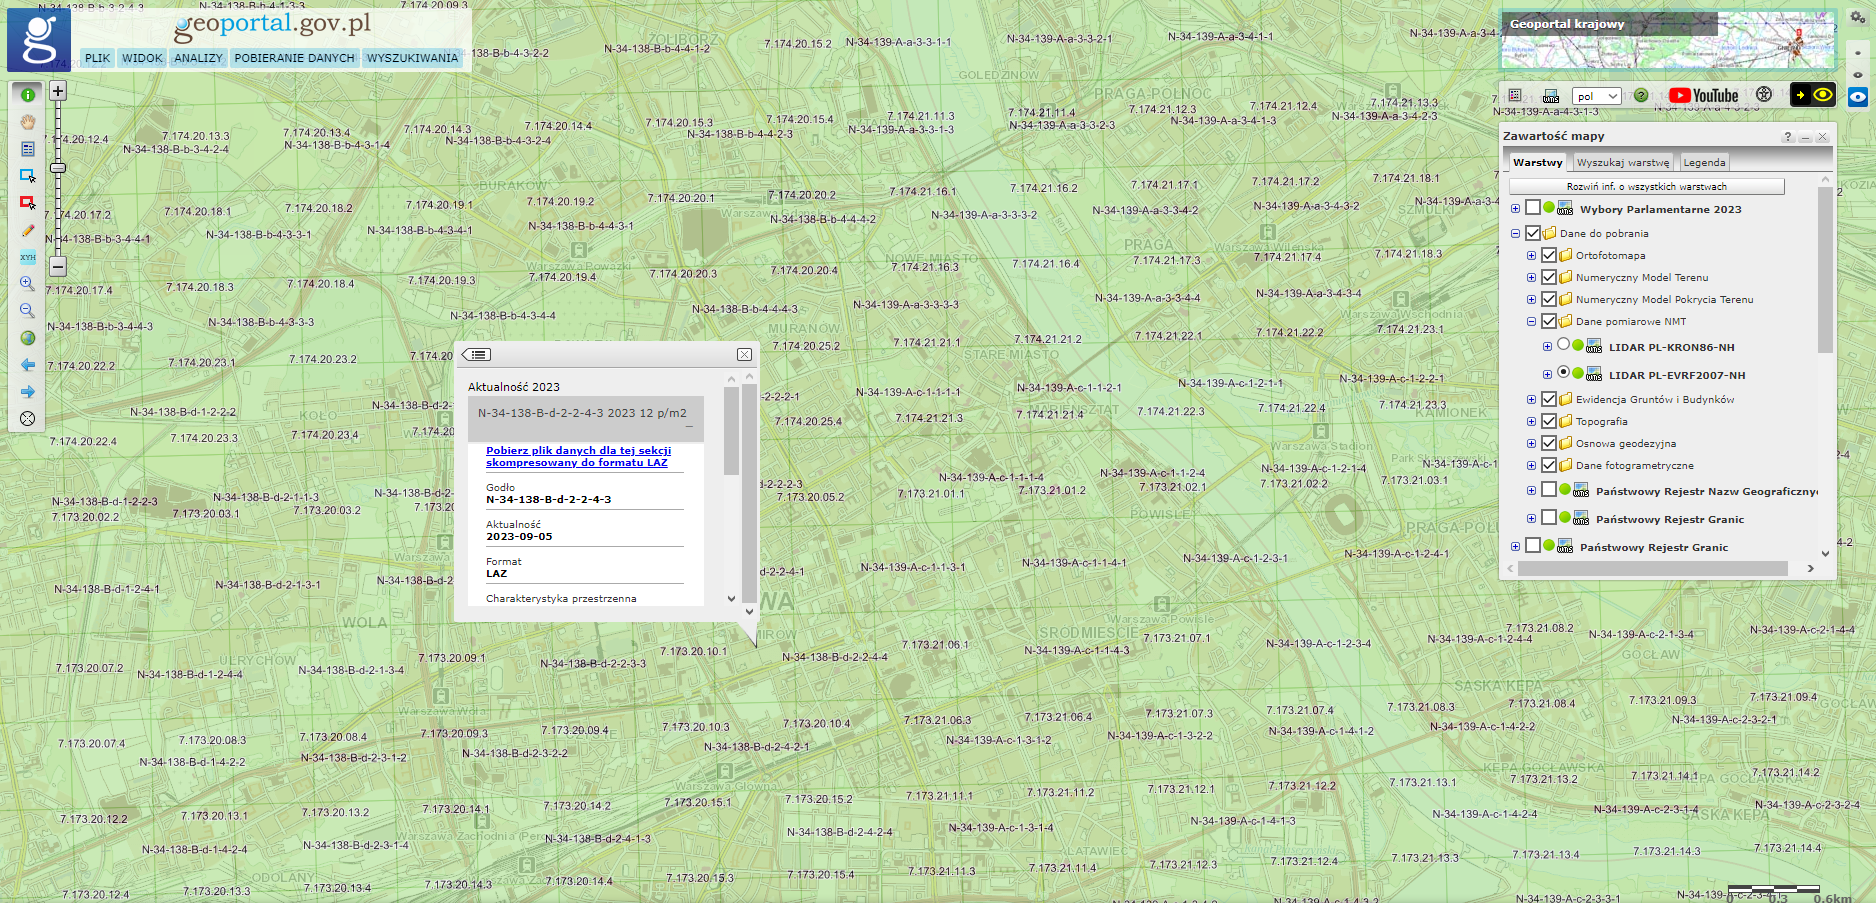
\includegraphics[width=\textwidth]{ISOK5.png}
	\caption{Then choose the newest version (usually the highest one) and use the link to download .laz file. Repeat this and previous step for every tile that covers your area of interest.}
	\label{fig:38}
\end{figure}

\begin{figure}[H]
	\centering
	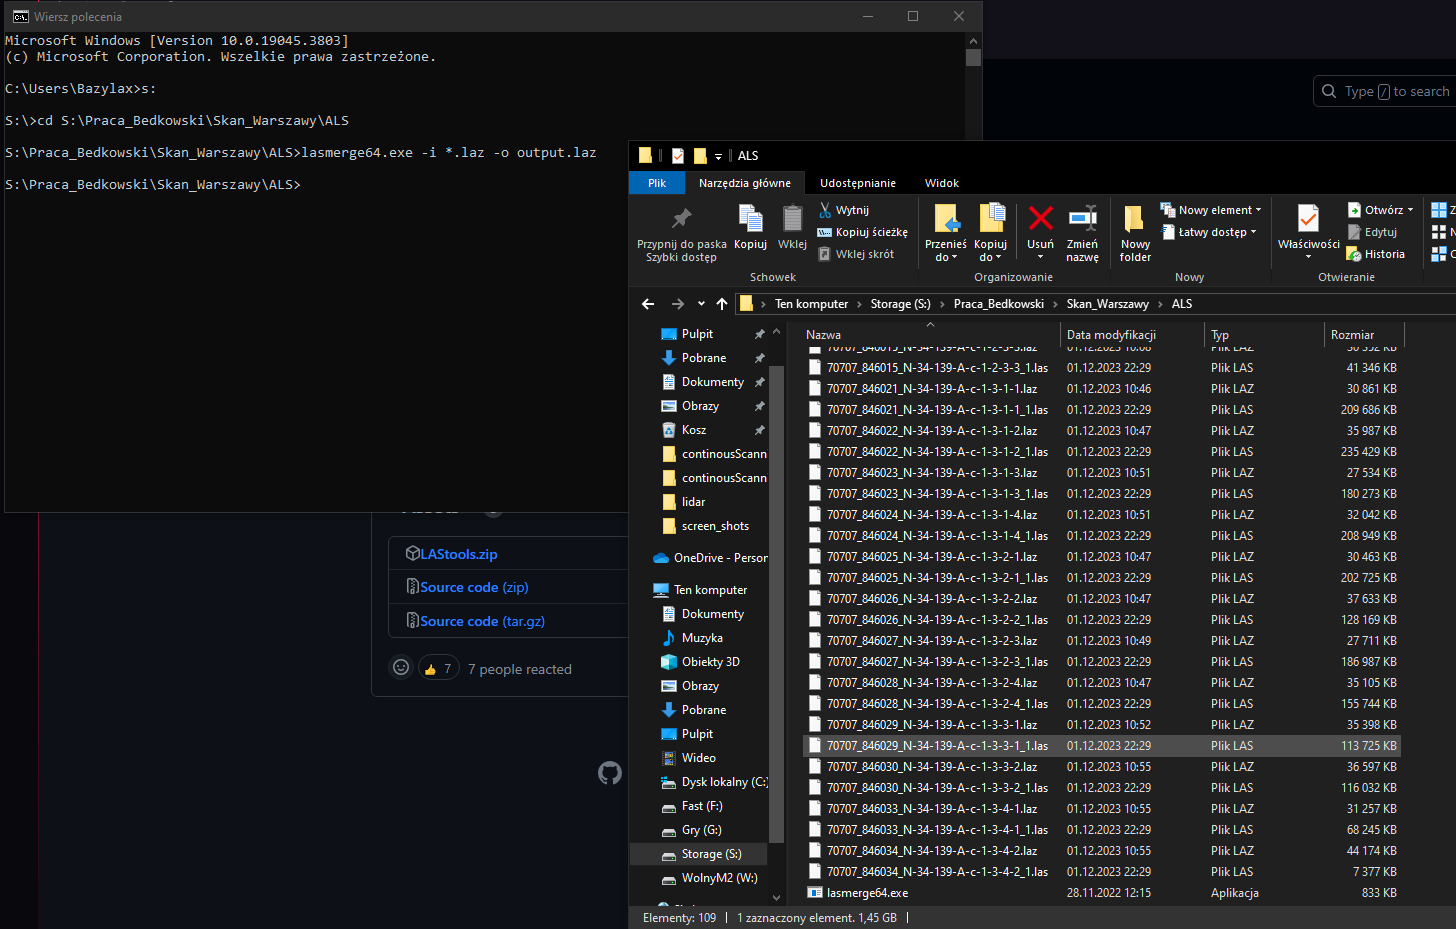
\includegraphics[width=\textwidth]{ISOK6.png}
	\caption{If merging of downloaded tiles is needed, I recommend using LAStools software. Download LAStools.zip from release page (\url{https://github.com/LAStools/LAStools/releases}). From folder bin/ extract lasmerge64.exe and put it in the folder where tile .laz files are stored. Open windows command prompt, move to directory with .laz files and write command: 
		\textit{lasmerge64.exe -i *.laz -o <your output .laz file name>.laz}}
	\label{fig:39}
\end{figure}

\begin{figure}[H]
	\centering
	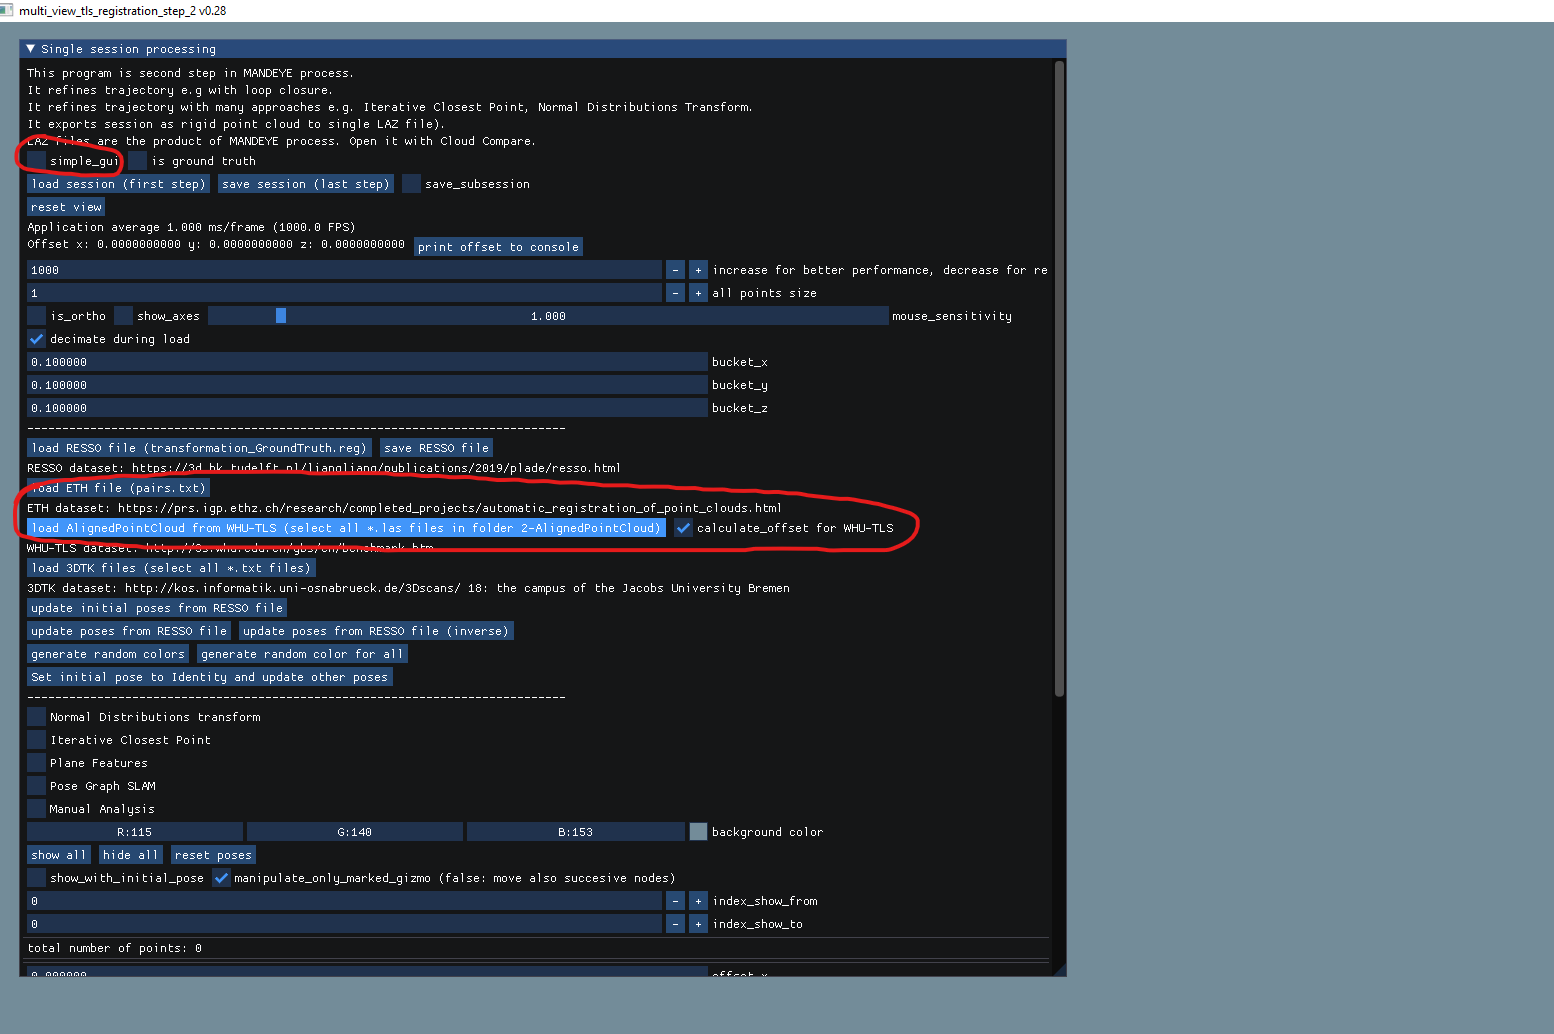
\includegraphics[width=\textwidth]{ISOK7.png}
	\caption{Open step 2 of this manual (\ref{fig:10}), unmatch simple gui, select calculate offset and load WHU-TLS data (many laz./las. files may be chosen).}
	\label{fig:40}
\end{figure}

\begin{figure}[H]
	\centering
	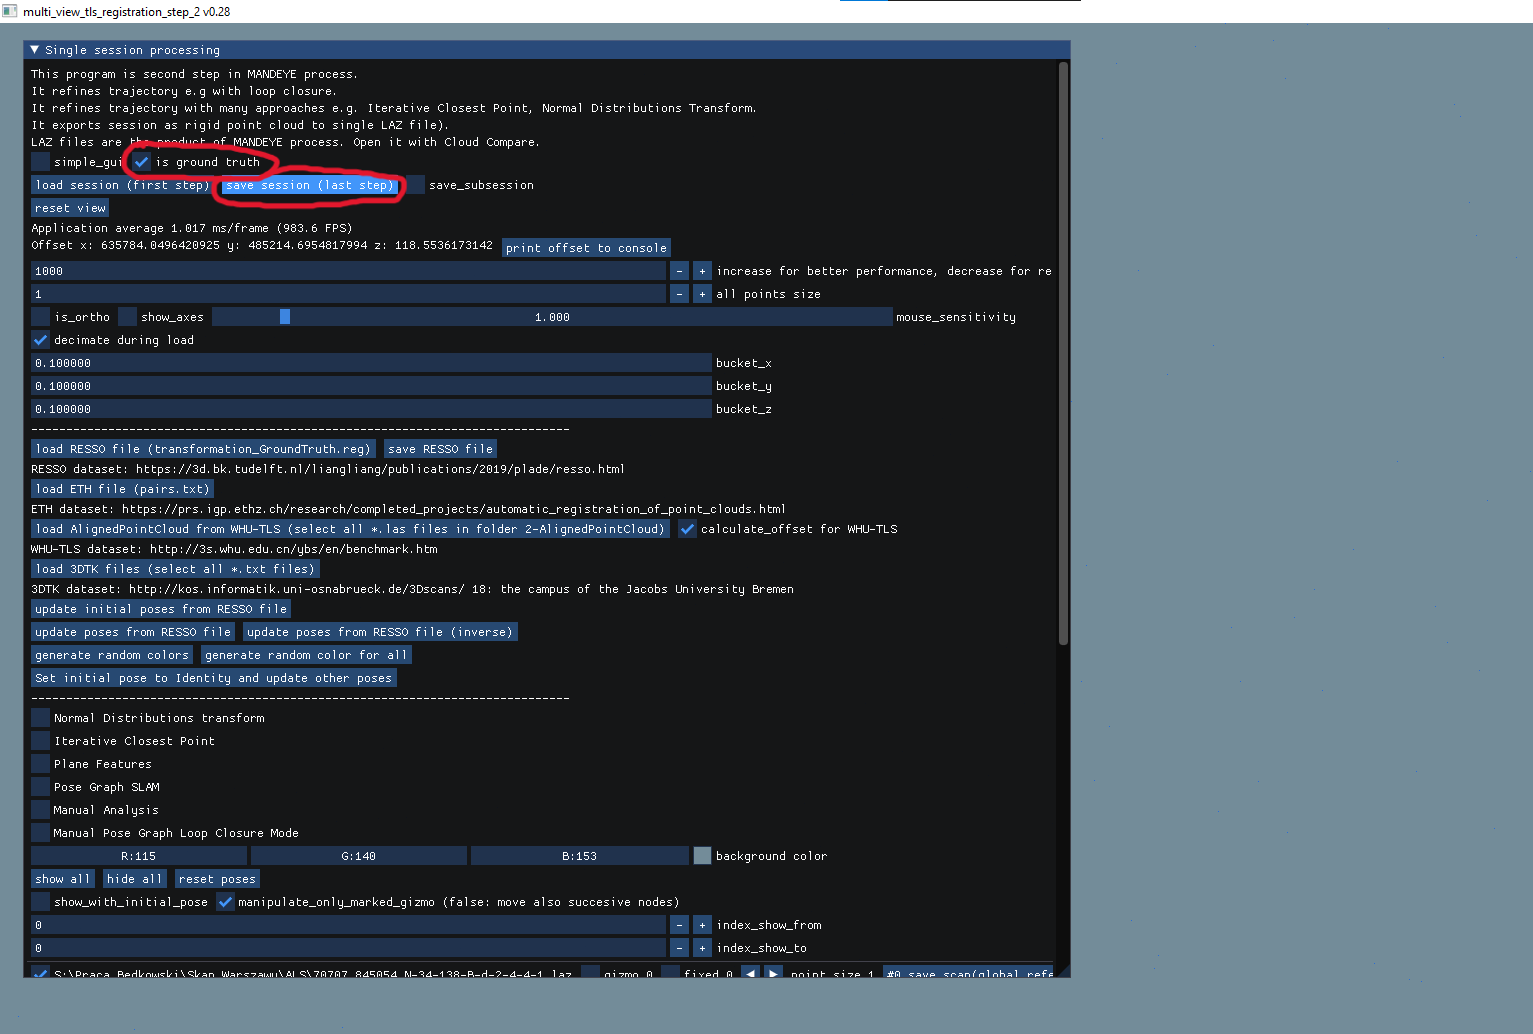
\includegraphics[width=\textwidth]{ISOK8.png}
	\caption{After loading scans successfully check ground truth option and save session as new .json file that contains all loaded scans. Now these scans may be loaded to serve as ground truth session that other scans can be aligned to.}
	\label{fig:41}
\end{figure}

\section{Georeferencing with ground control points (GCP)}
\label{GCPs}
Prepare at least 3 ground control points with e.g. GPS receiver (Longitude, Latitude, Altitude), see figures \ref{fig:GCP1}, \ref{fig:GCP2}, \ref{fig:GCP3}.
Prepare GCP in local coordinate system using arbitrary chosen projection, thus each one has x, y, z coordinates.
Please apply offset to GSPs and store it to export data in global coordinate system.
%You can align session to 

During survey please place MANDEYE on top of each GCP (for at least 30 seconds) that LiDAR xy center will be exactly in the xy center of GCP (see figures \ref{fig:GCP4} and \ref{fig:GCP5}).
The resulting trajectory should be as shown in figure \ref{fig:trj}.
Measure LiDAR optic center height above ground as shown in figure \ref{fig:GCP6}.
Adding GCPs to the system is done via trajectory node picking (see figure \ref{fig:picking}).
First, check box 'Show ground control point gui' in 'Single session processing' window.
Second, check box 'picking trajectory node and adding GCP mode'.
Third, read GUI help and pick GCP corresponding node of the trajectory with middle mouse button and pressing 'ctrl'.
Fourth, add GCP observation to the system by clicking 'Add Ground Control Point' (see figure \ref{fig:addgcp}).
Now it is possible to change GCP name, uncertainty (sigma x, sigma y, sigma z), coordinates (x, y, z) and LiDAR height above ground.
Now it is time to manual transformation of the trajectory using GIZMO (see figures \ref{fig:gcp1} and \ref{fig:gcp2}). 
Uncheck 'manipulate only marked gizmo' to move all nodes of the trajectory that all GPCs are in proper positions.
You can save session to json to store all GPS in the project file.

Important notice: starting from v0.59 you can align session to all GCPs with button 'Register session to Ground Control Points (trajectory is rigid)' placed in the end of GUI window 'Ground Control Point'.
This functionality is preserving the shape of the trajectory, thus the consecutive relative poses will not change.  
It is recommended to use it before applying 'Manual Pose Graph Loop Closure Mode'.

All GPCs are considered in 'Manual Pose Graph Loop Closure Mode', so they will converge assuming assigned uncertainty. 
To export point cloud to global reference system applied offset has to be provided in GUI (see figure \ref{fig:offset}).
Thus, for all point the offset transformation will applied during export.

\begin{figure}[H]
	\centering
	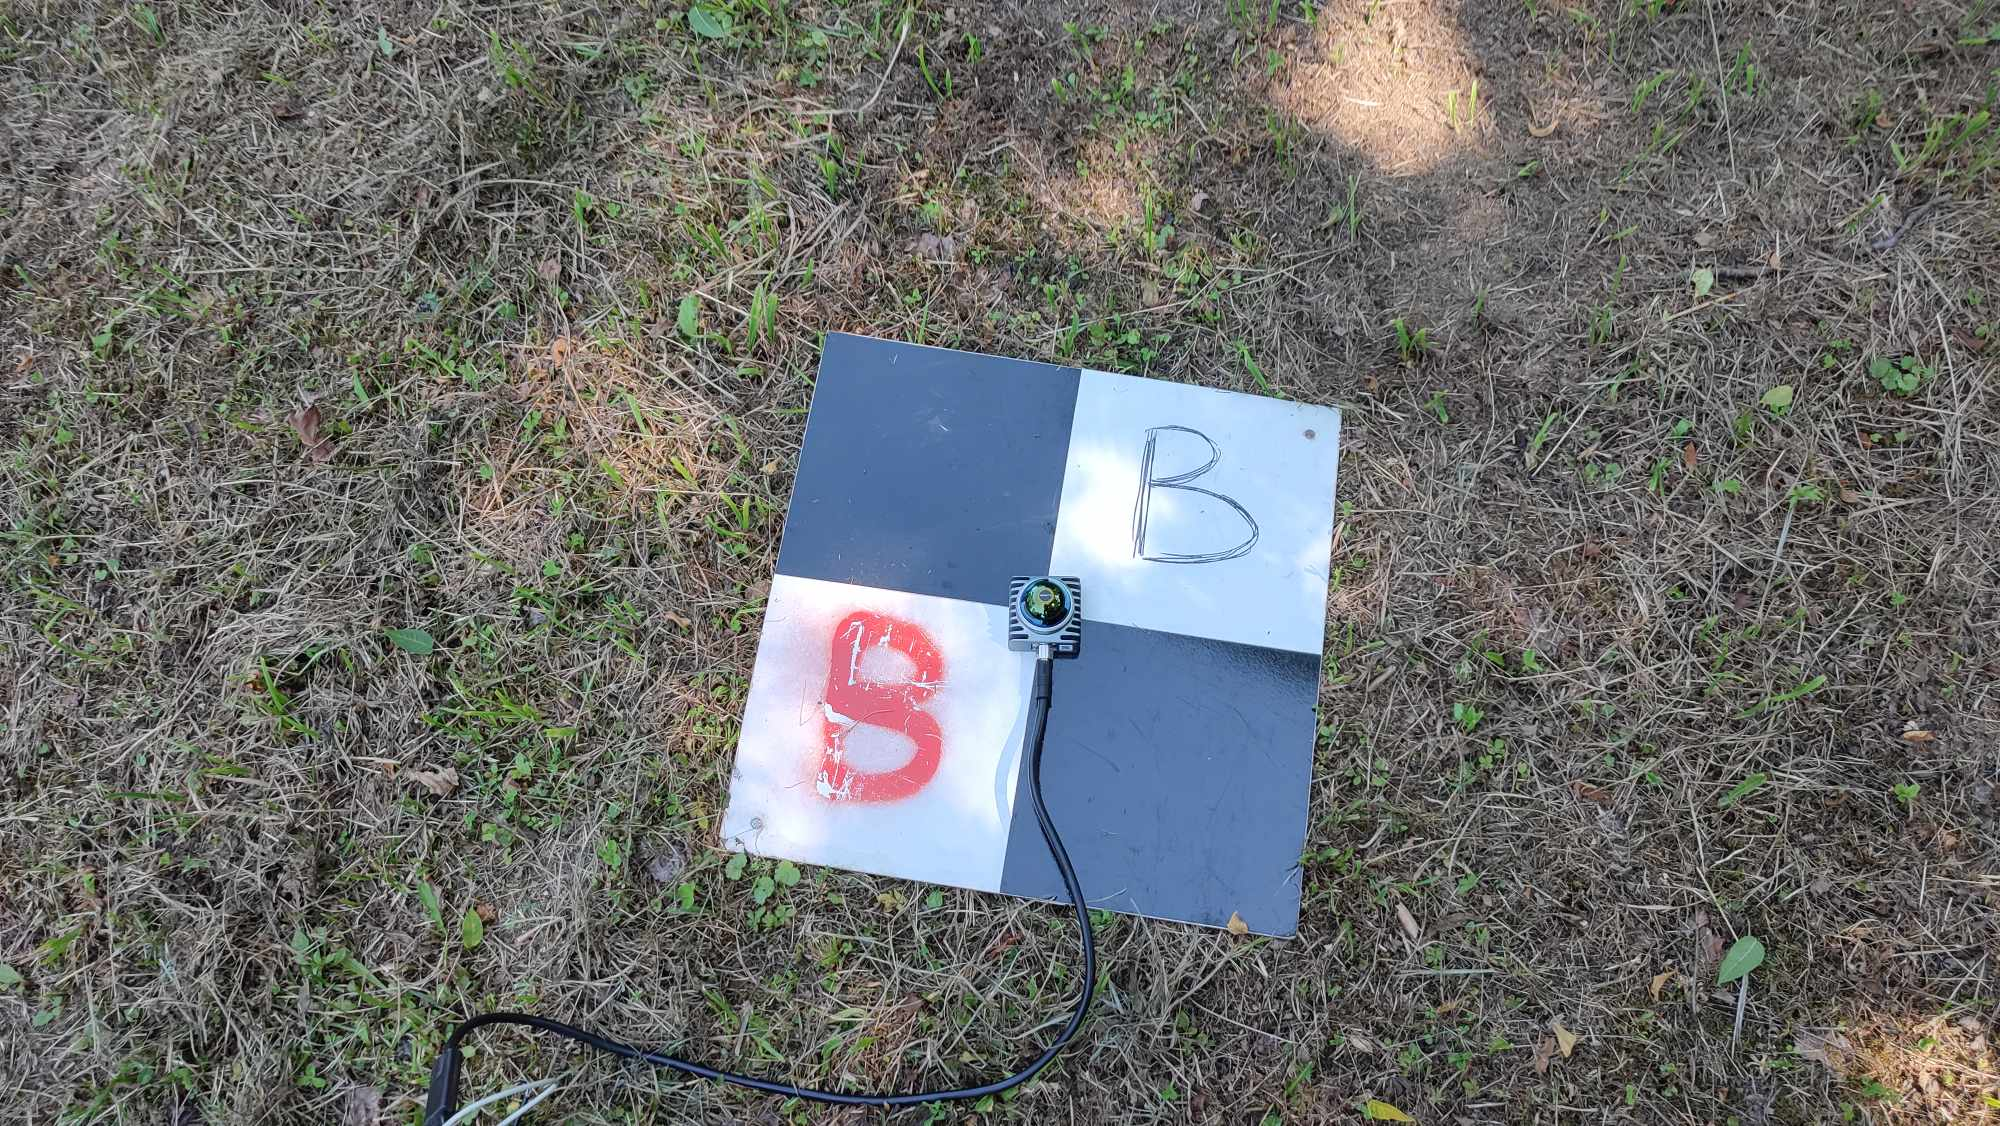
\includegraphics[width=\textwidth]{0137d3b0-79f7-4e83-98f8-d4a5737f573b.jpeg}
	\caption{Ground control points - example 1.}
	\label{fig:GCP1}
\end{figure}

\begin{figure}[H]
	\centering
	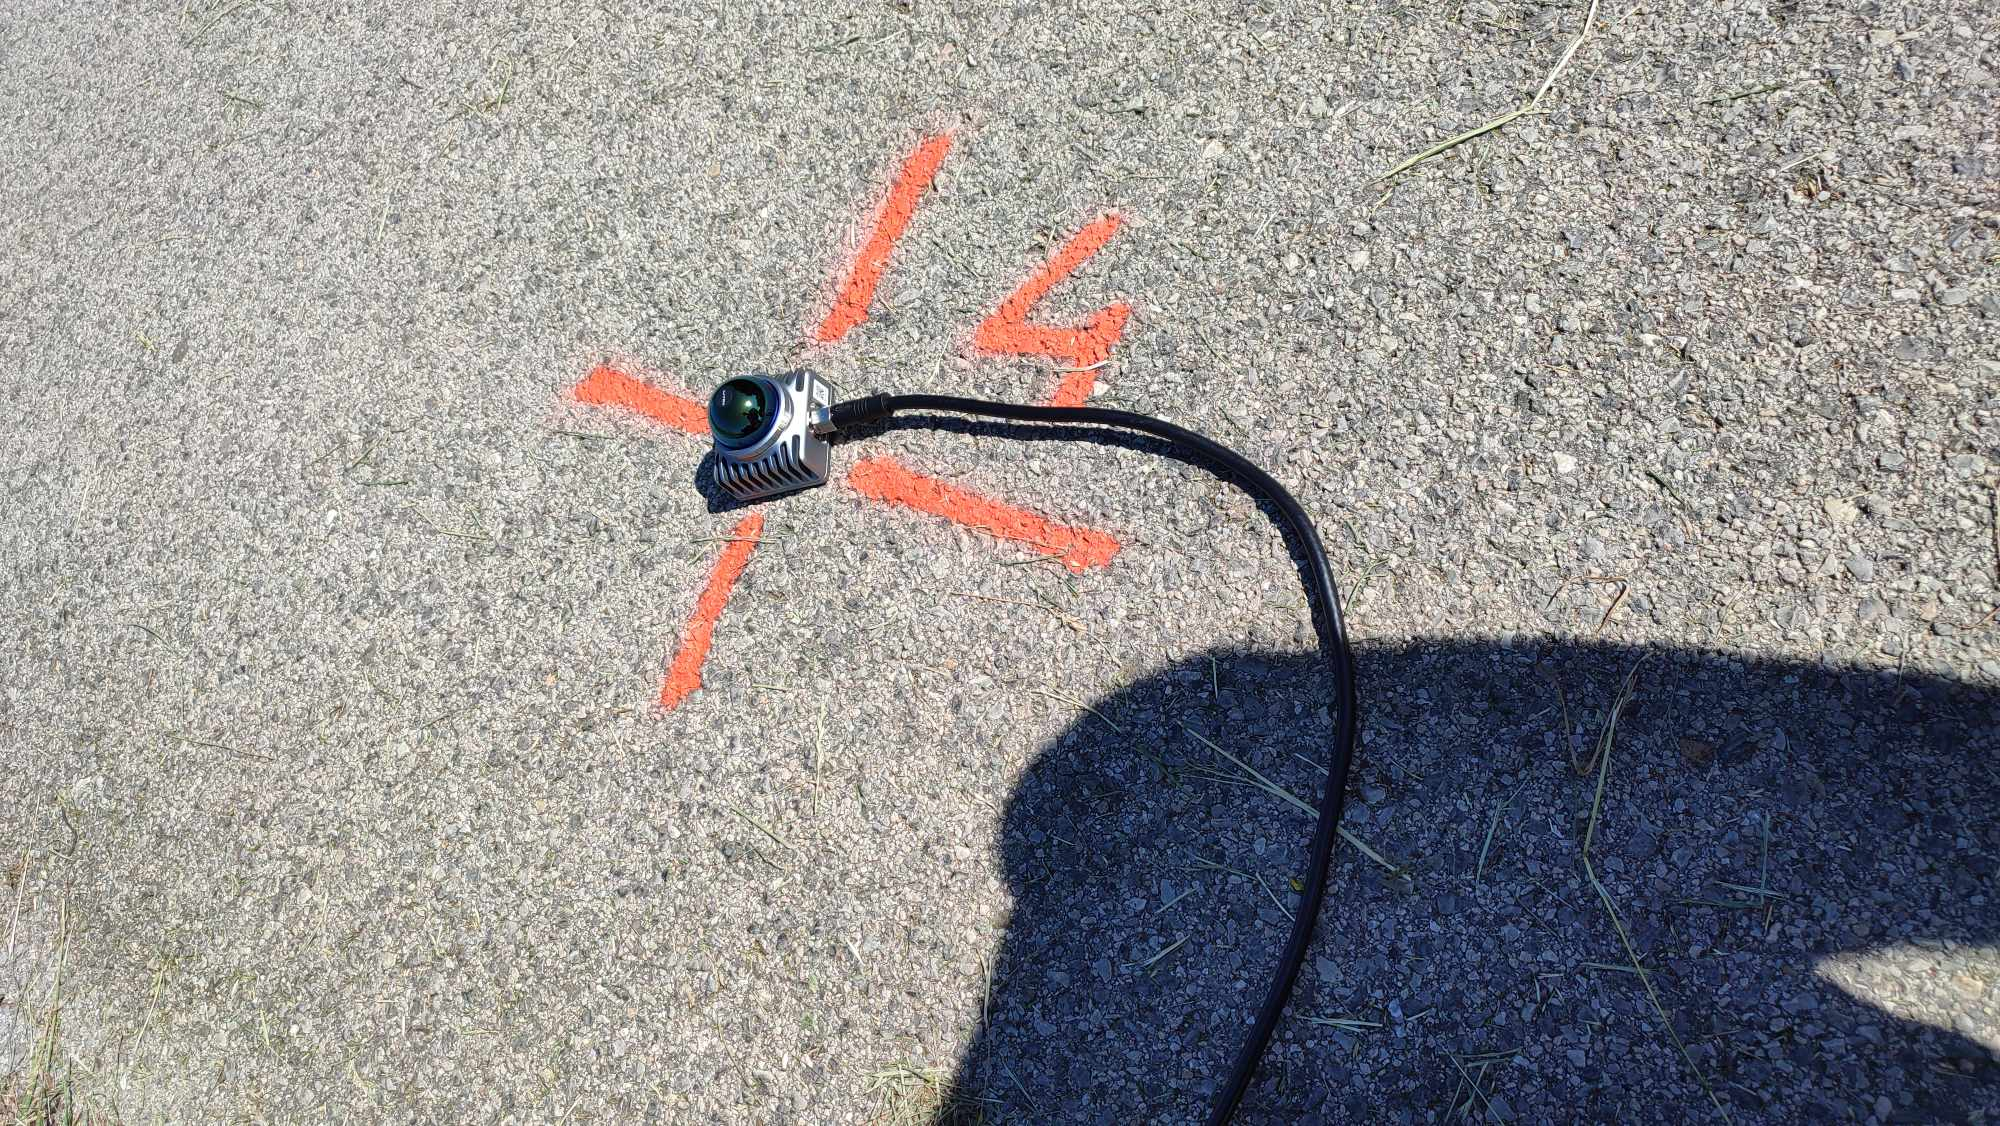
\includegraphics[width=\textwidth]{e02cbef6-16e1-43c4-86fd-ac824ed8dc9f.jpeg}
	\caption{Ground control points - example 2.}
	\label{fig:GCP2}
\end{figure}

\begin{figure}[H]
	\centering
	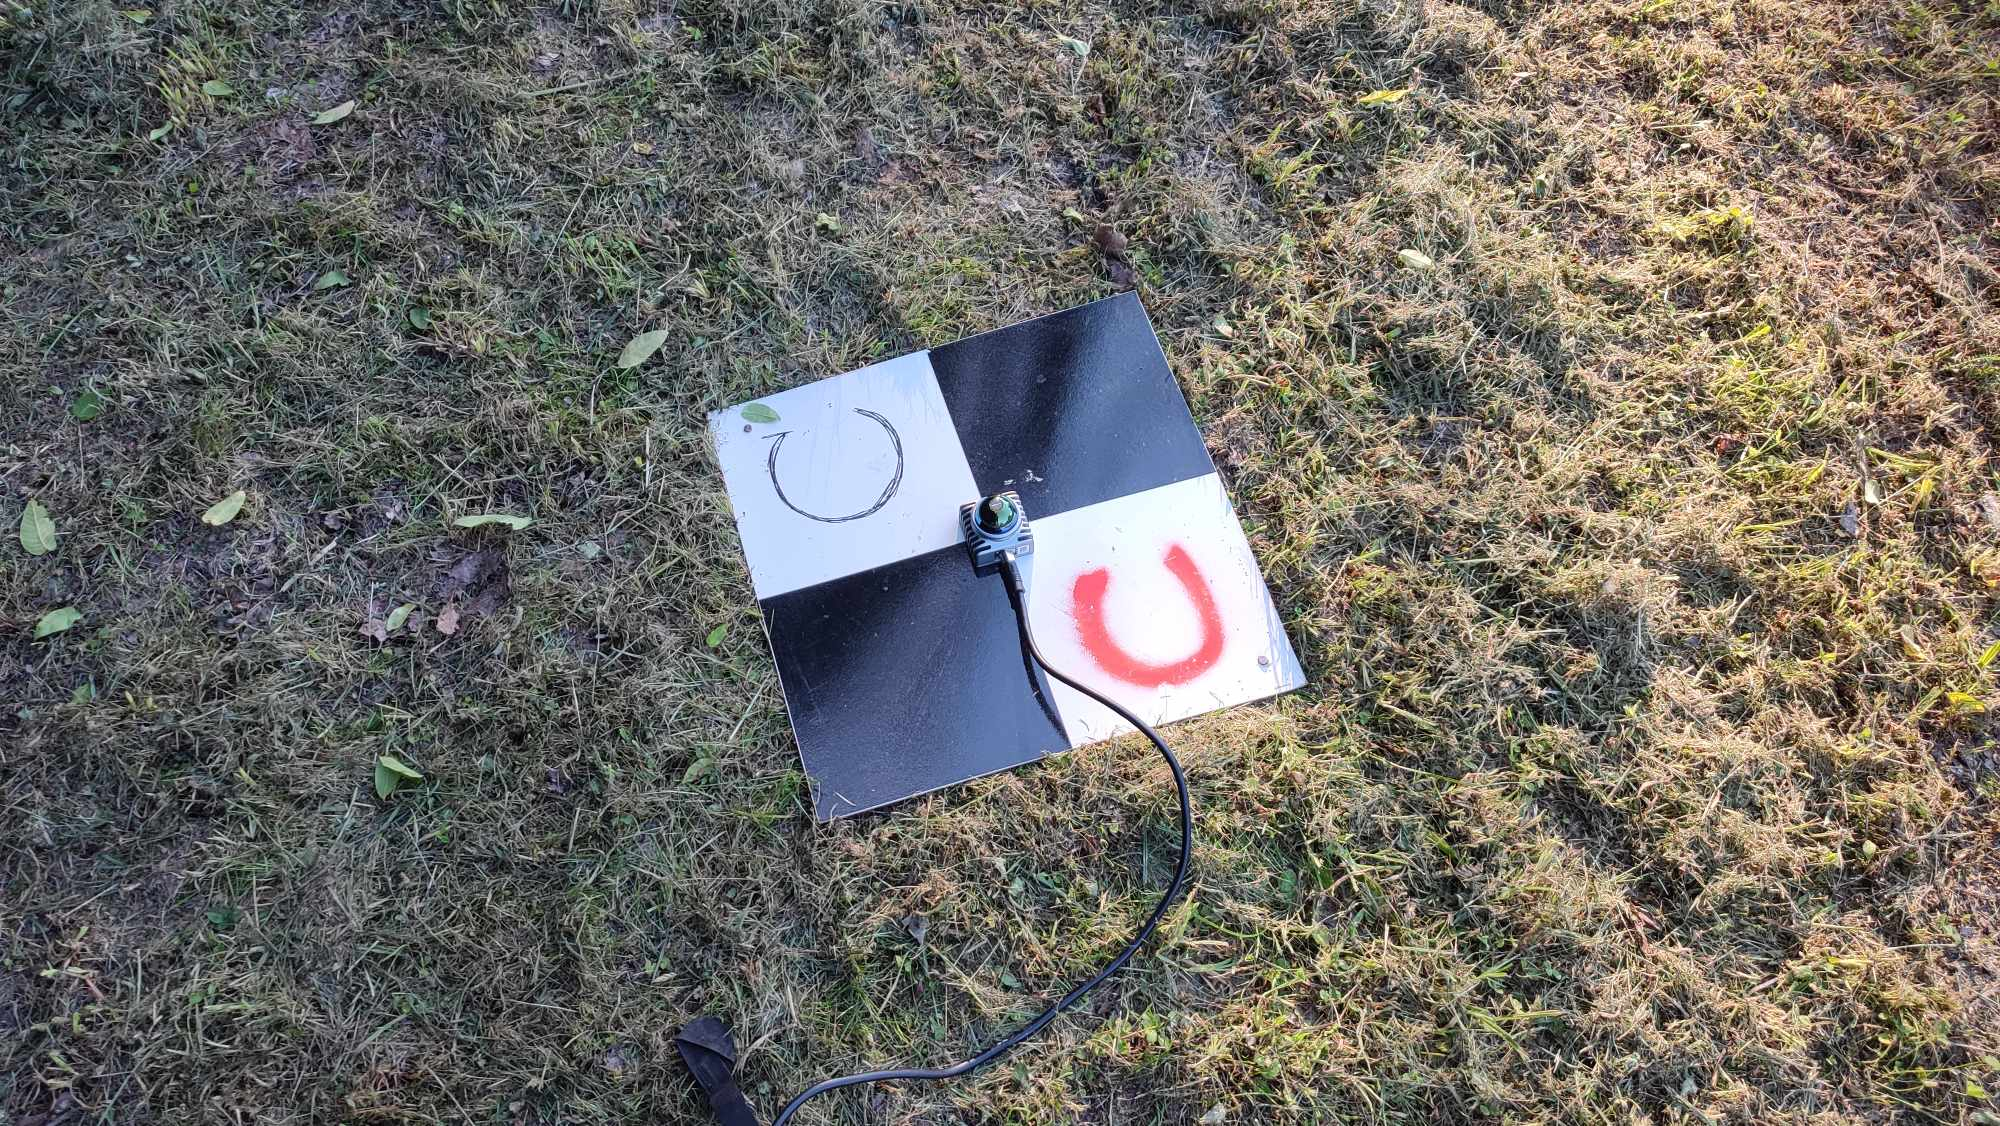
\includegraphics[width=\textwidth]{e5c6464b-4e01-4560-b464-c316ffd281db.jpeg}
	\caption{Ground control points - example 3.}
	\label{fig:GCP3}
\end{figure}

\begin{figure}[H]
	\centering
	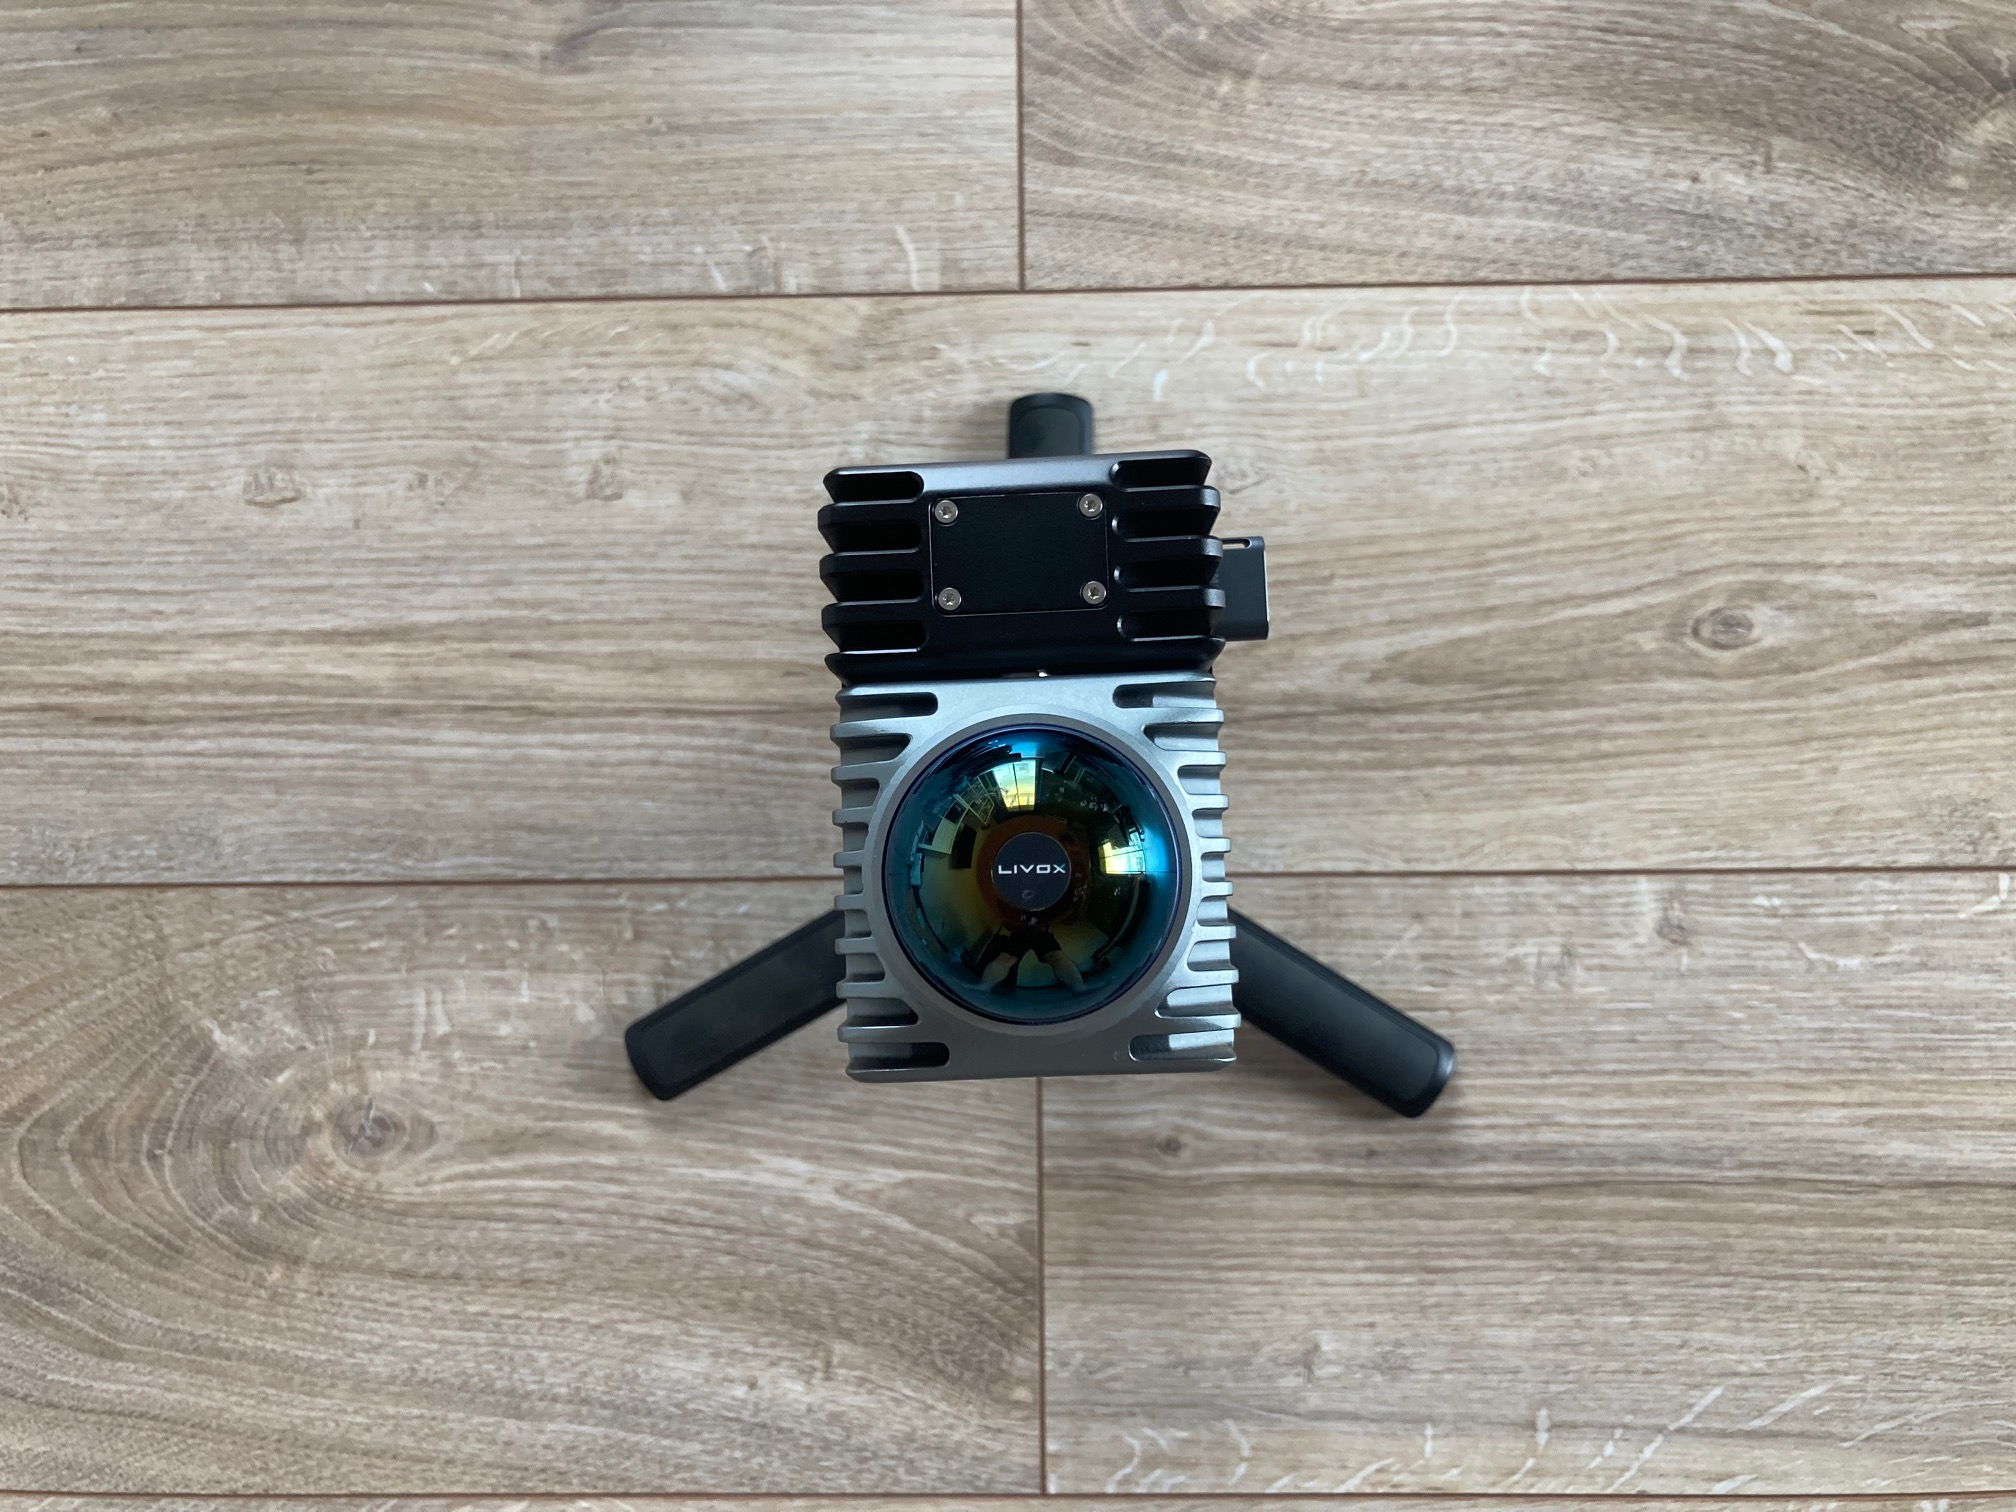
\includegraphics[width=\textwidth]{IMG_1123.png}
	\caption{LiDAR xy center is exactly in the xy center of GCP.}
	\label{fig:GCP4}
\end{figure}

\begin{figure}[H]
	\centering
	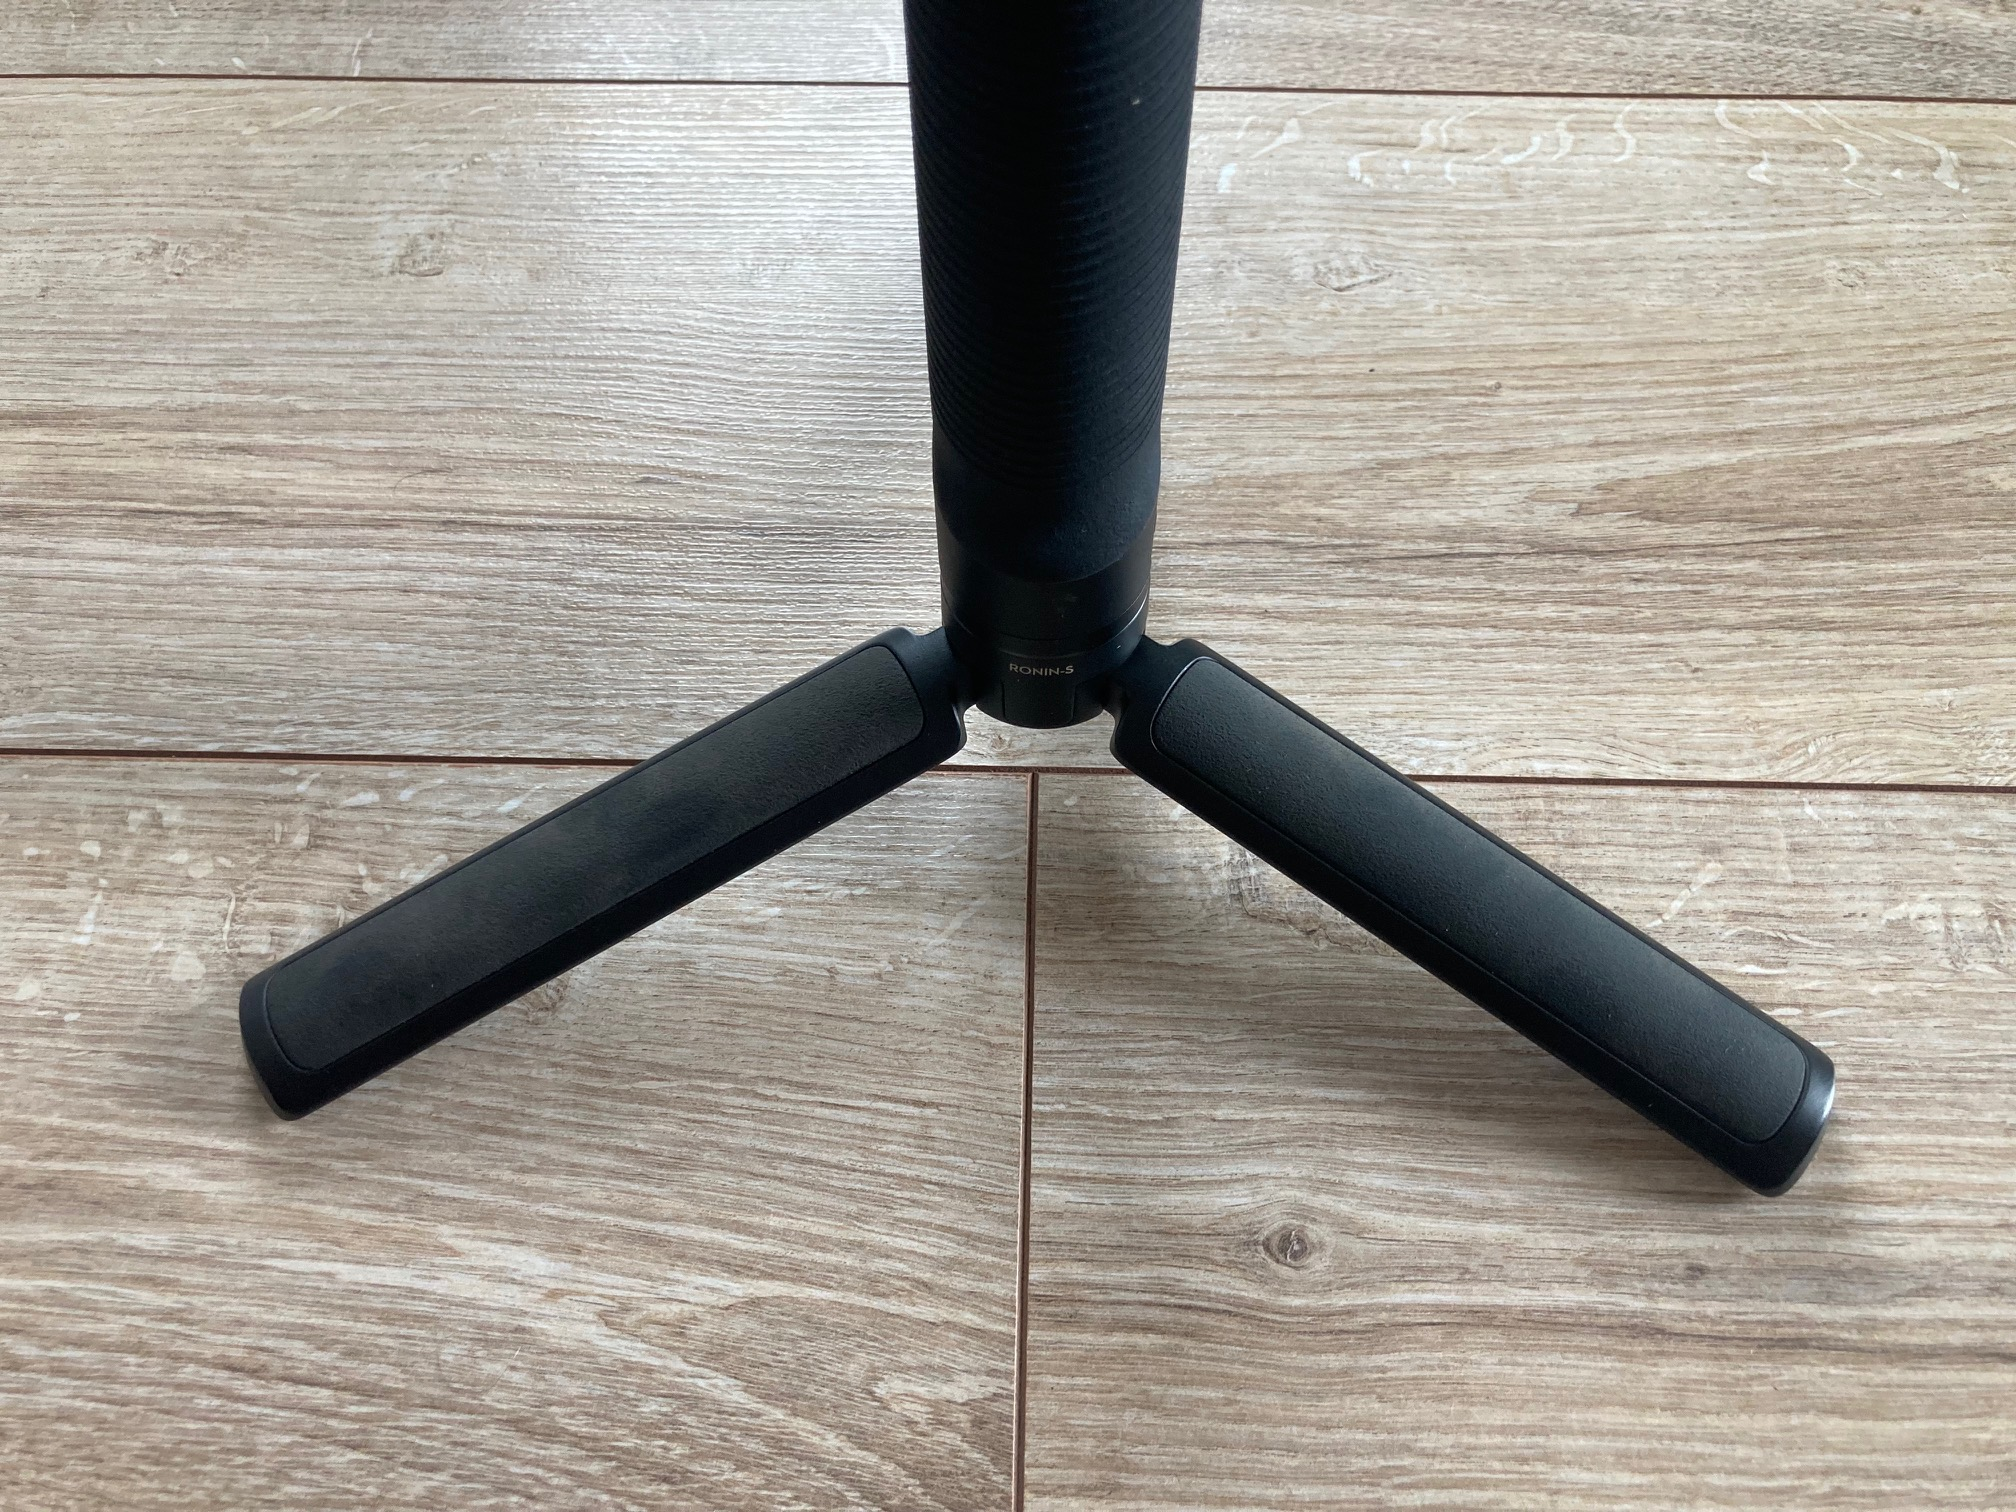
\includegraphics[width=\textwidth]{IMG_1124.png}
	\caption{LiDAR xy center is exactly in the xy center of GCP.}
	\label{fig:GCP5}
\end{figure}

\begin{figure}[H]
	\centering
	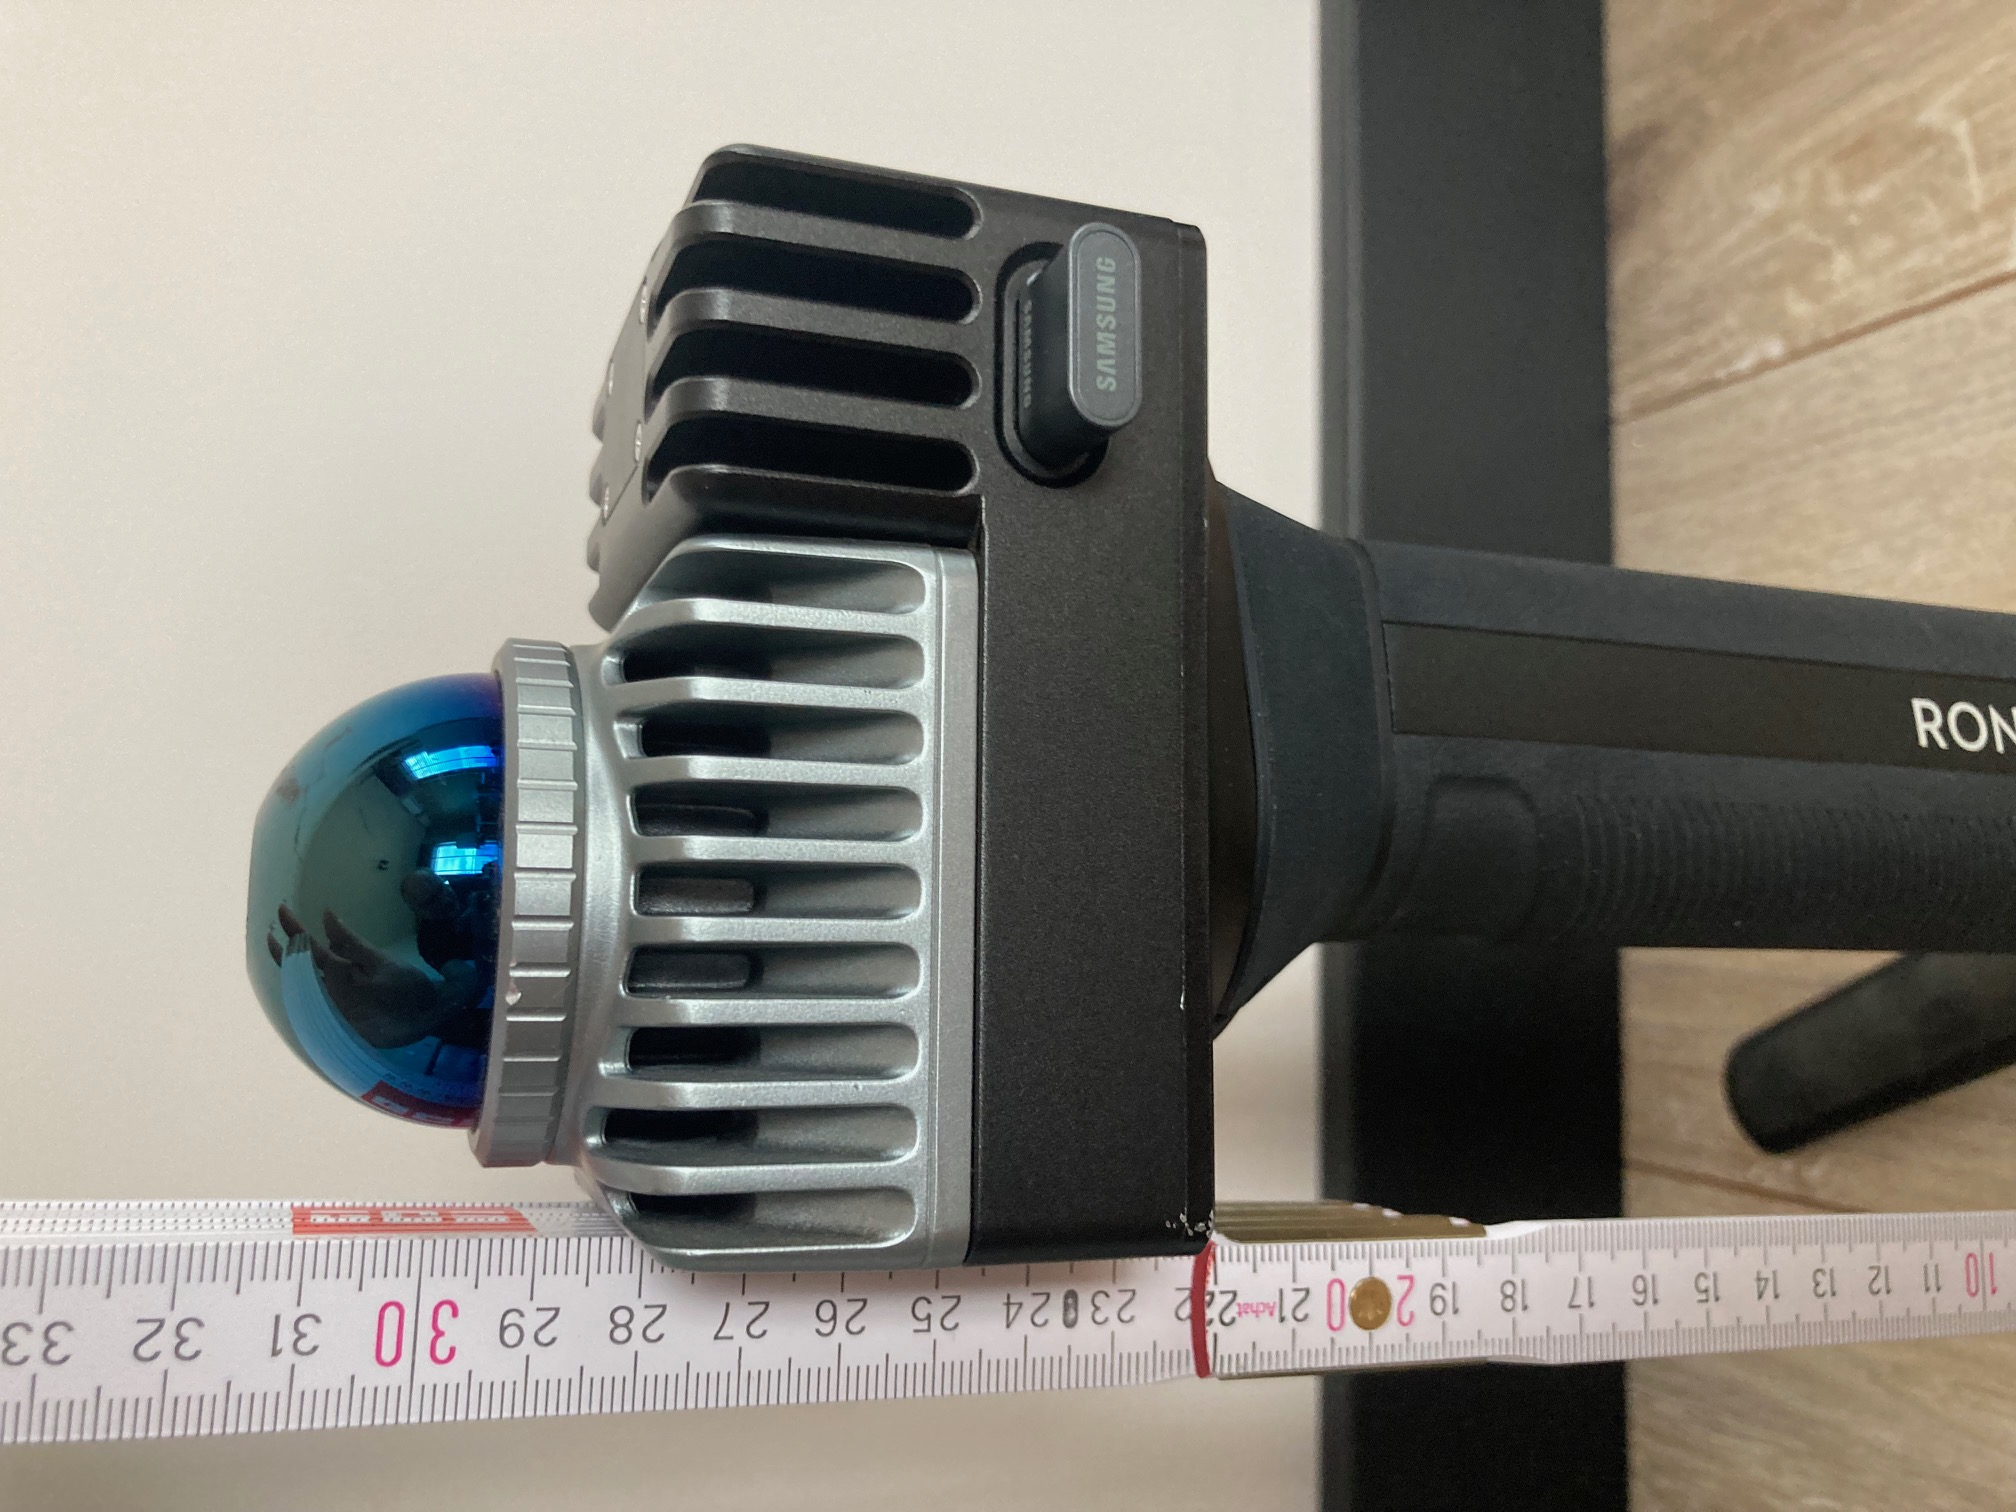
\includegraphics[width=\textwidth]{IMG_1122.png}
	\caption{Measurement of LiDAR optic center height above ground (GCP ground plane).}
	\label{fig:GCP6}
\end{figure}

\begin{figure}[H]
	\centering
	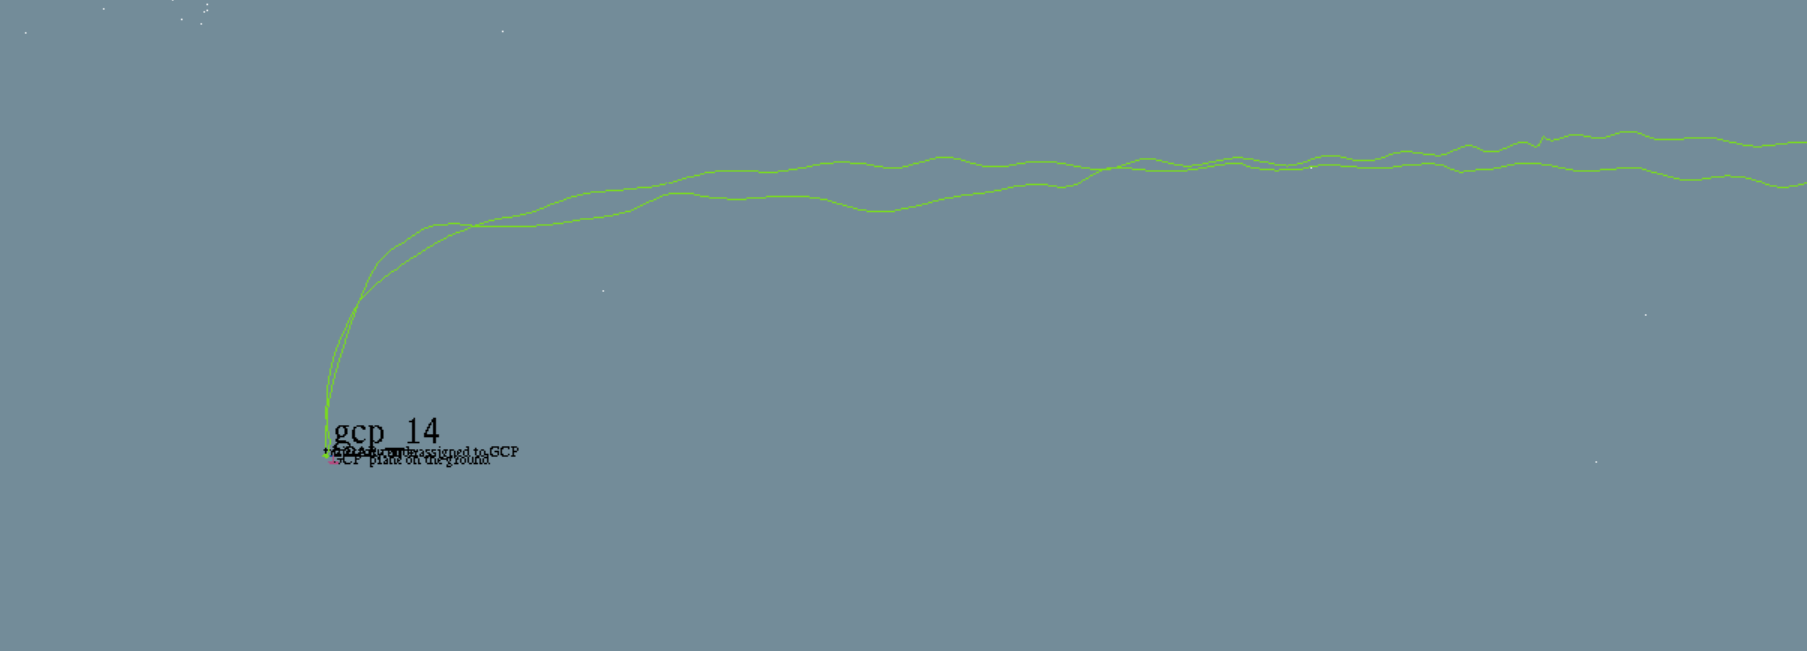
\includegraphics[width=\textwidth]{trj.png}
	\caption{Trajectory with ground control point. }
	\label{fig:trj}
\end{figure}

\begin{figure}[H]
	\centering
	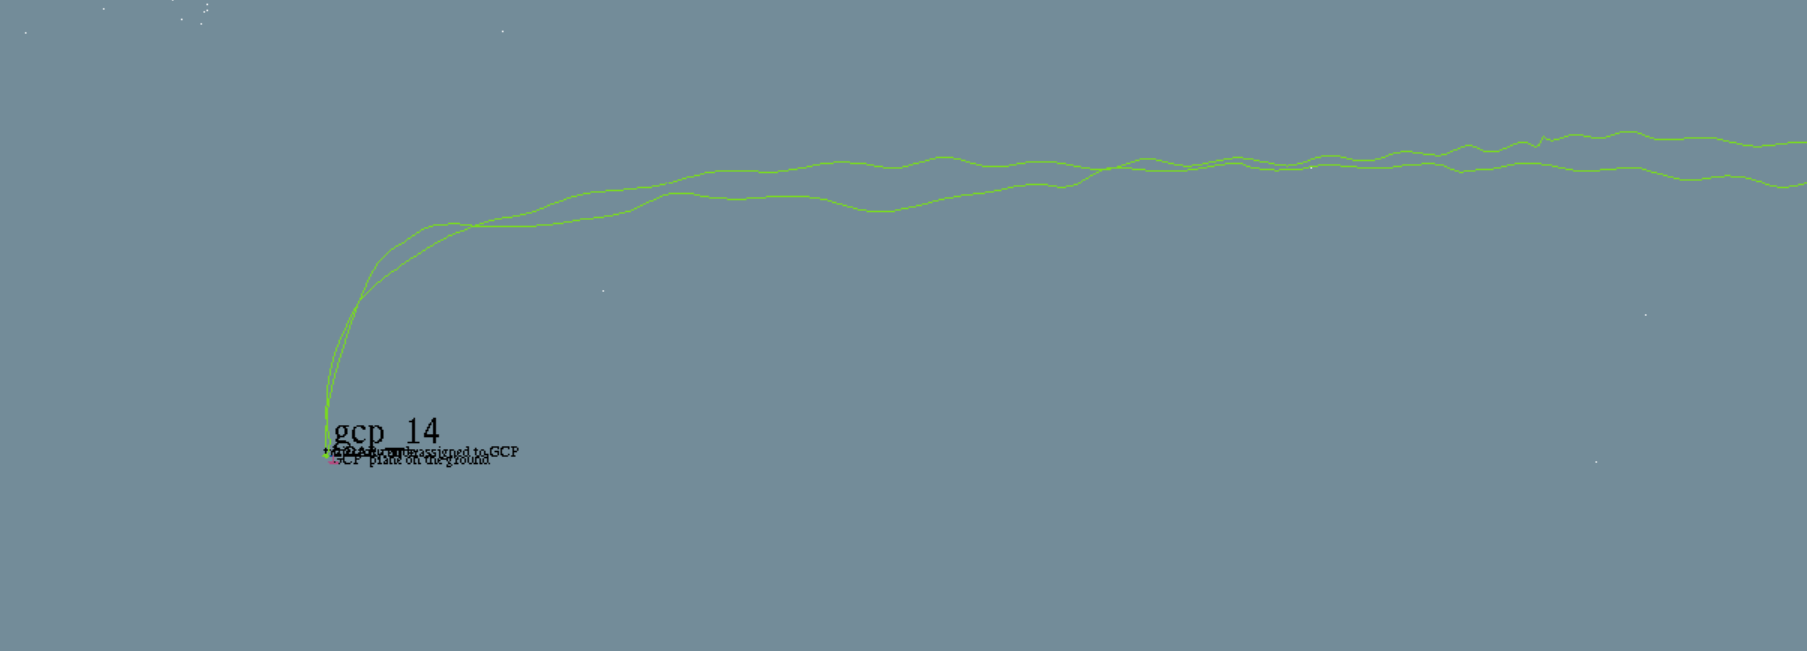
\includegraphics[width=\textwidth]{trj.png}
	\caption{GCP picking.}
	\label{fig:picking}
\end{figure}

\begin{figure}[H]
	\centering
	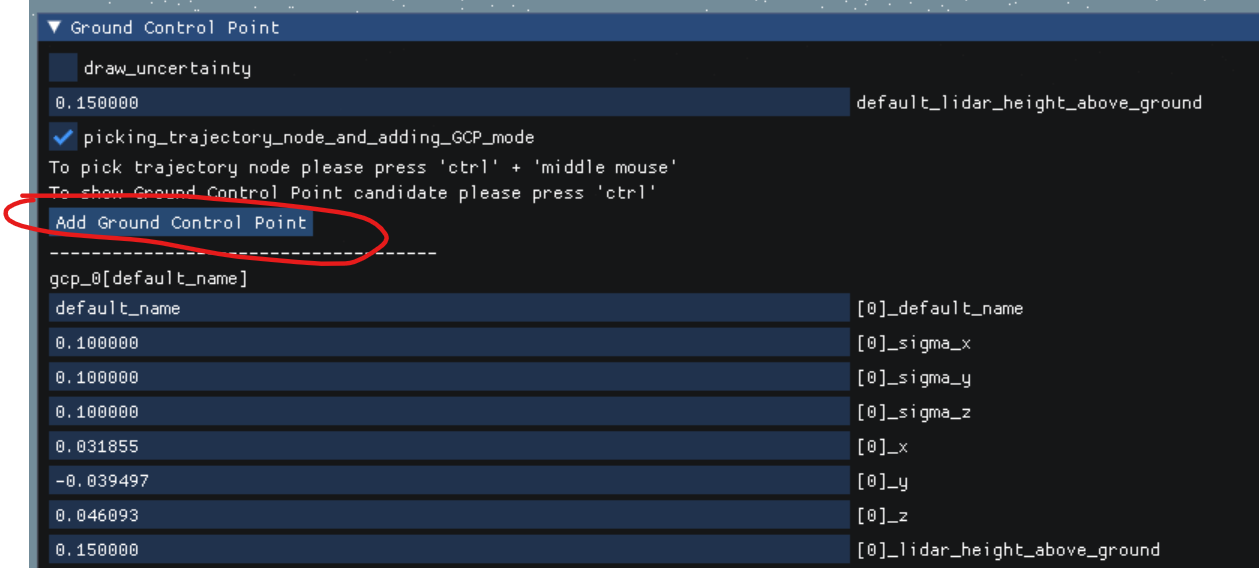
\includegraphics[width=\textwidth]{addgcp.png}
	\caption{Adding GCP observation.}
	\label{fig:addgcp}
\end{figure}

\begin{figure}[H]
	\centering
	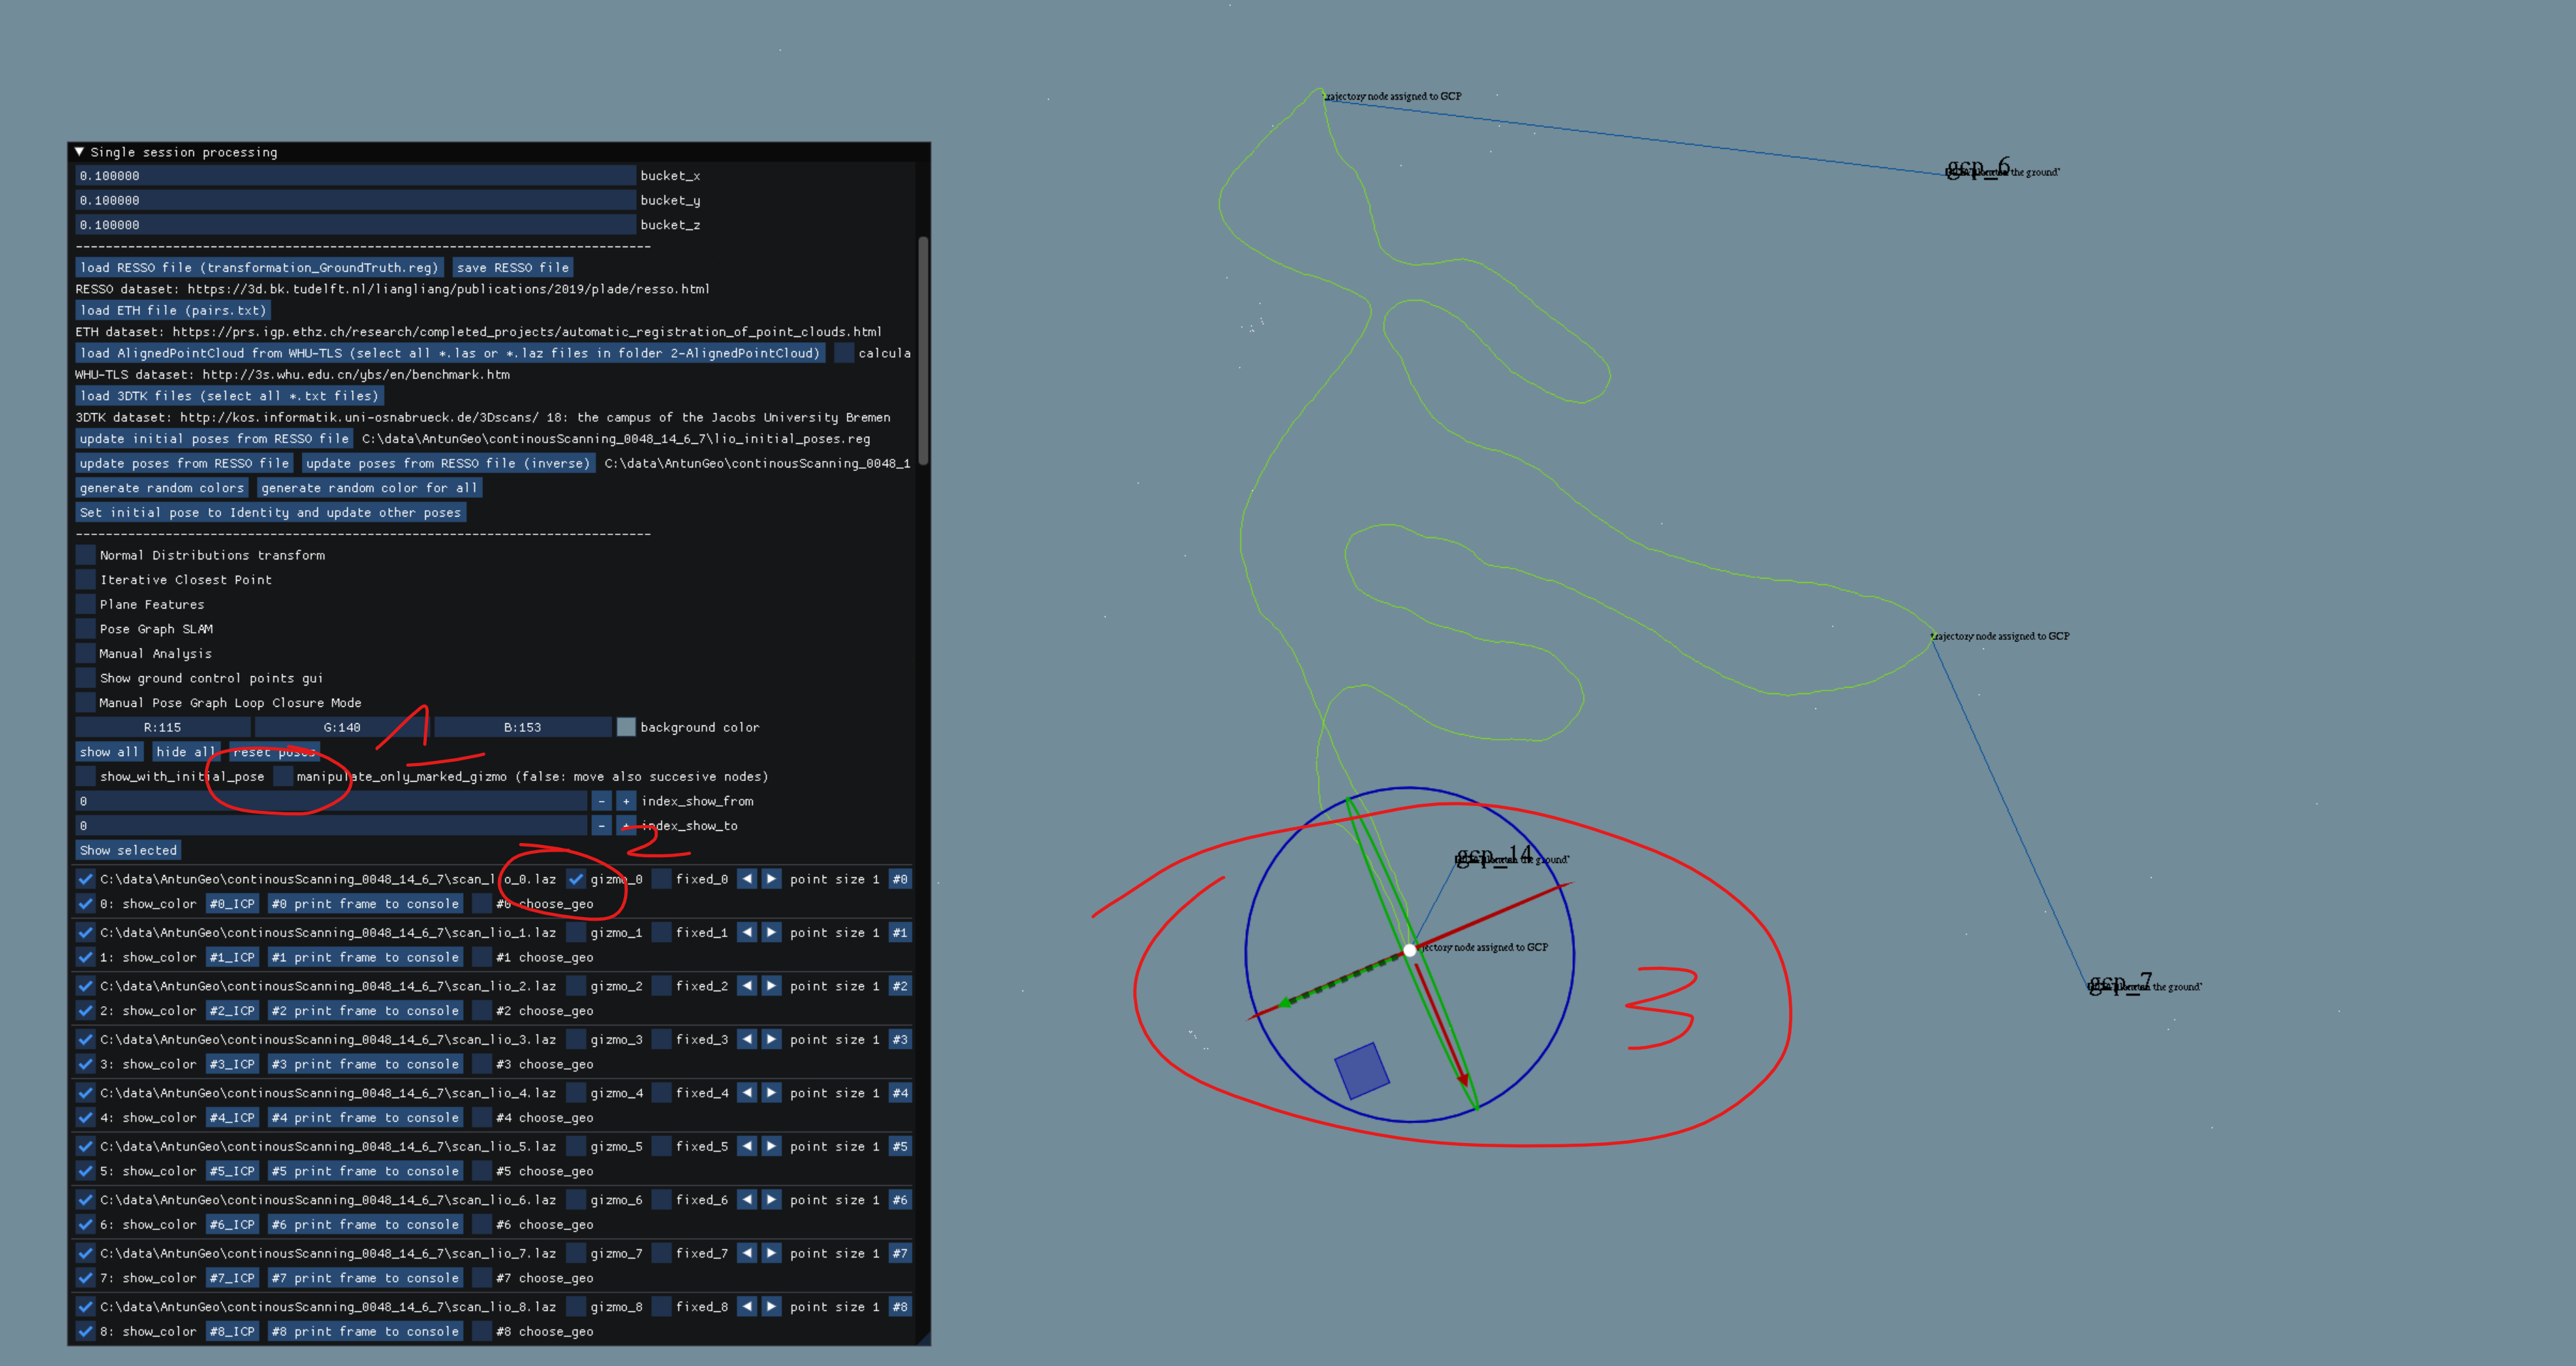
\includegraphics[width=\textwidth]{gcp1.png}
	\caption{Manual transformation of the trajectory using GIZMO (un-check manipulate only marked gizmo to move all nodes of the trajectory).}
	\label{fig:gcp1}
\end{figure}

\begin{figure}[H]
	\centering
	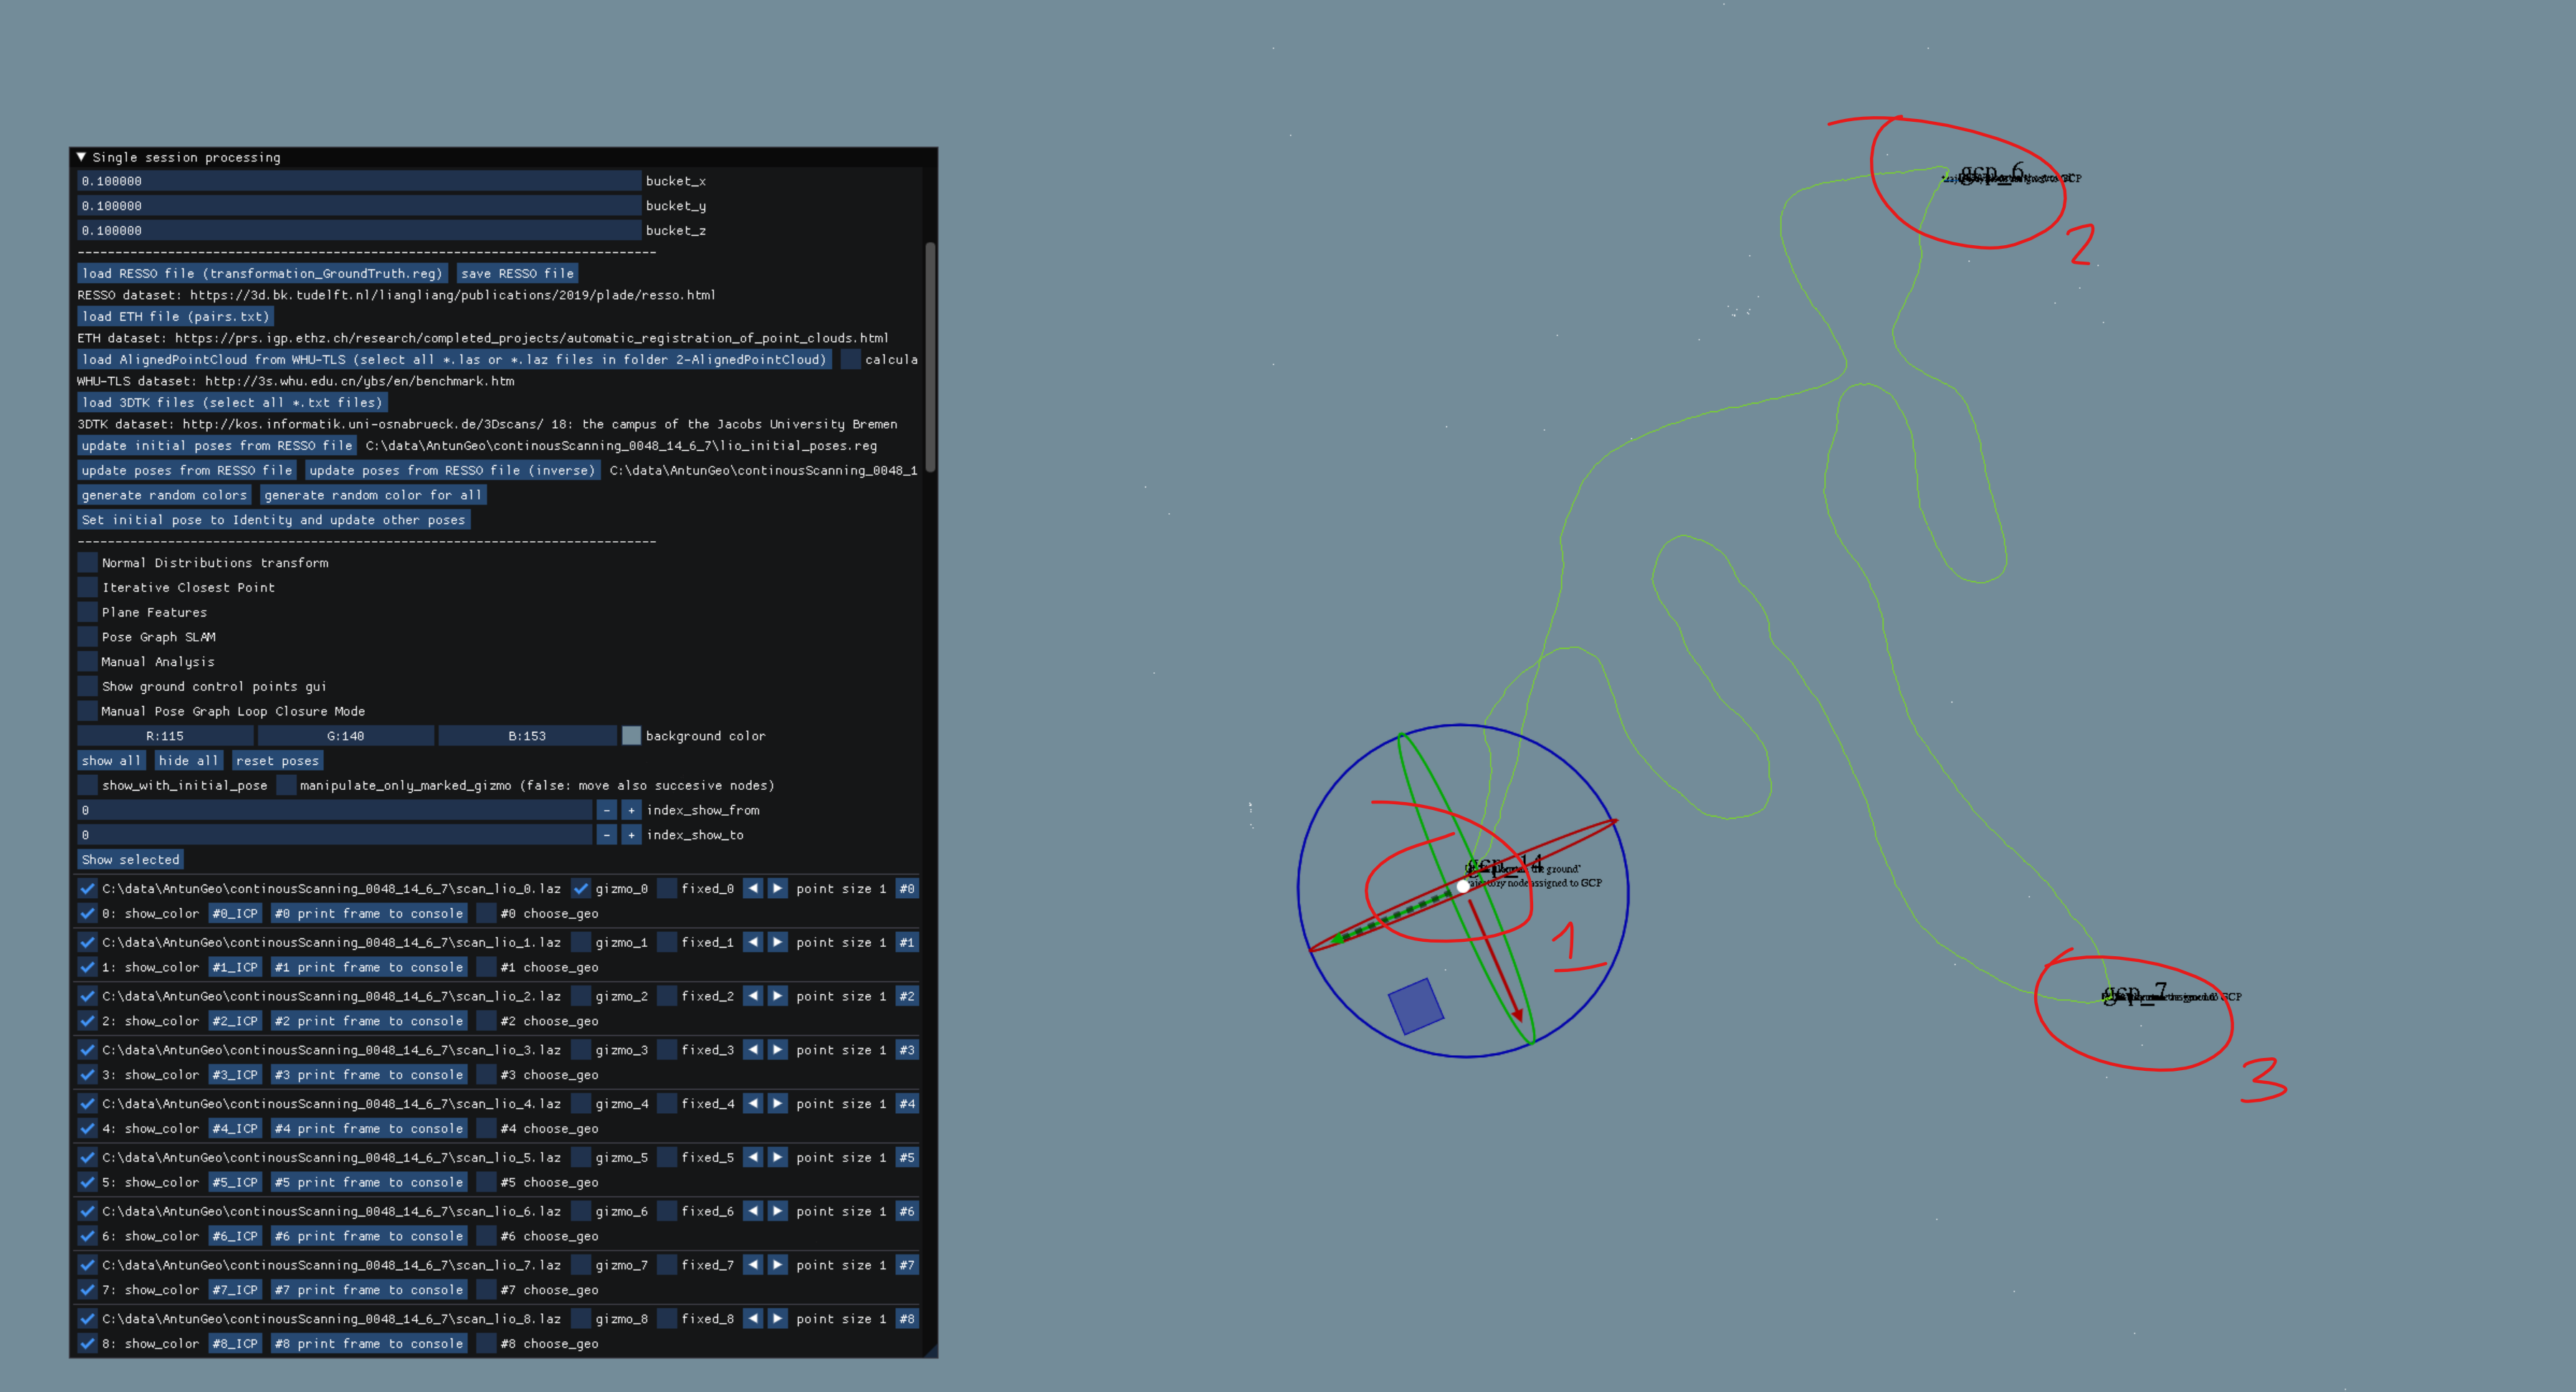
\includegraphics[width=\textwidth]{gcp2.png}
	\caption{Found proper transformation GCPs to trajectory nodes.}
	\label{fig:gcp2}
\end{figure}

\begin{figure}[H]
	\centering
	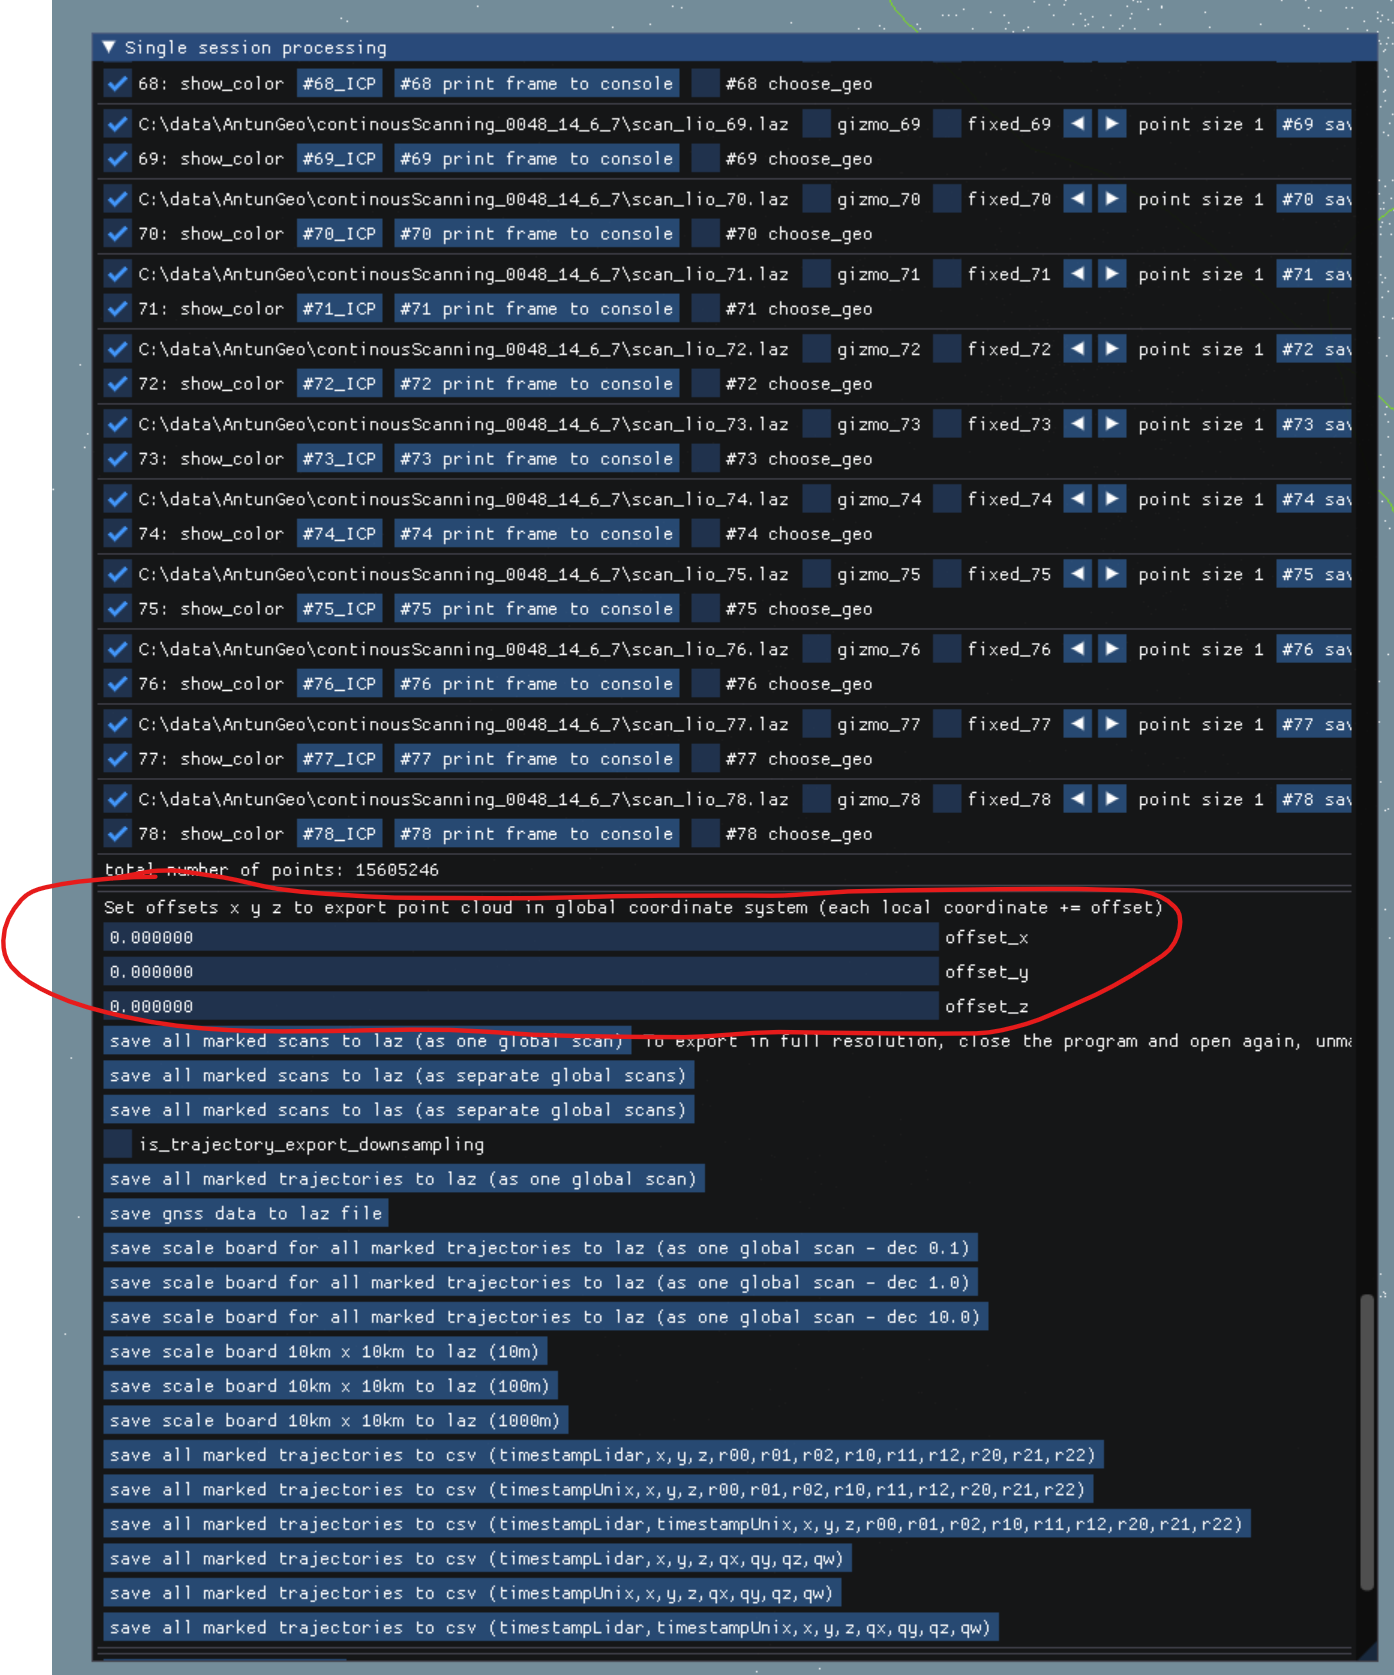
\includegraphics[width=\textwidth]{offset.png}
	\caption{Applying offset to export point cloud in global reference system.}
	\label{fig:offset}
\end{figure}


